\section{Visualization Details and Discussion}
\label{sec:supp-visualization}

\begin{figure}[t]
	\centering
	\vspace*{-0.2cm}
	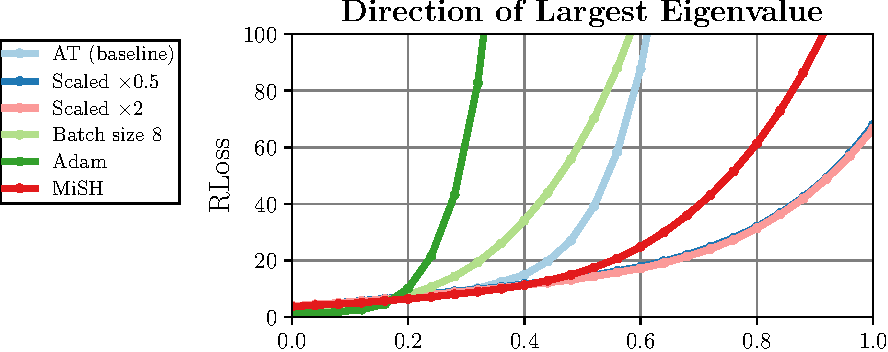
\includegraphics[width=0.425\textwidth]{plots_supp_hessian}
	\vspace*{2px}
	
	\hspace*{-0.35cm}
	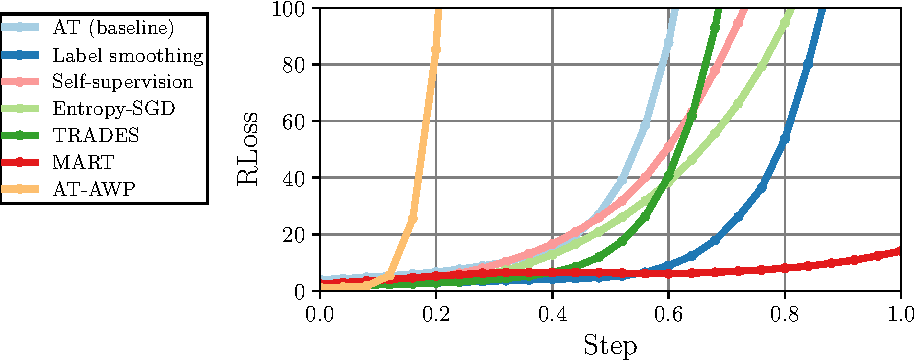
\includegraphics[width=0.44\textwidth]{plots_supp_hessian2}
	\vspace*{-4px}
	\caption{\textbf{Visualization in ``Hessian'' Direction:} \RCE visualized in the direction of the largest Hessian eigenvalue (\ie, the corresponding eigenvector). The eigenvalues quantify the ``rate of change'' along the corresponding eigenvector. Thus, the largest eigenvalue represents a worst-case direction in weight space. Clearly, \RCE increases significantly in these directions.}
	\label{fig:supp-visualization}
	\vspace*{-6px}
\end{figure}

\textbf{Visualization Details:}
%
For the plots in the main paper, we compute the mean \RCE across $10$ random, normalized directions; for adversarial directions, we plot max \RCE over $10$ adversarial directions. After normalization, we re-scale the weight directions to have length $0.5$ for random directions and $0.025$ for adversarial directions. This essentially ``zooms in'' and is particularly important when visualizing along adversarial weight directions. In all cases, we estimate \RCE on one batch of $128$ test examples for $51$ evenly spaced  step sizes in $[-1, 1]$. We found that using more test examples does not change the \RCE landscape significantly. \figref{fig:supp-visualization} shows additional visualizations along the direction of the largest Hessian eigenvalue (also using per-layer normalization, multiplied by $0.5$).

\textbf{Discussion of \cite{LiNIPS2018}:}
%
Originally, \cite{LiNIPS2018} uses a per-filter normalization instead of our per-layer normalization. Specifically, this means
\begin{align}
	\hat{\nu}^{(l,i)} &= \frac{\nu^{(l)}}{\|\nu^{(l,i)}\|_2} \|w^{(l,i)}\|_2\quad\text{ for layer }l\text{, filter }i,\label{eq:supp-normalization-filter}
\end{align}
instead of our normalization outlined in the main paper:
\begin{align}
	\hat{\nu}^{(i)} &= \frac{\nu^{(l)}}{\|\nu^{(l)}\|_2} \|w^{(l)}\|_2\quad\text{ for layer }l.\label{eq:supp-normalization}
\end{align}
Furthermore, \cite{LiNIPS2018} does not consider changes in the biases or batch normalization parameters. Instead, we also normalize the biases as above and take them into account for visualization (but not the batch normalization parameters). More importantly, \cite{LiNIPS2018} considers only (clean) \CE, while we focus on \RCE. Compared to the plots from the main paper, \figref{fig:supp-visualization-li} shows that the difference between filter-wise and layer-wise normalization has little impact in visually judging flatness. Generally, filter-wise normalization makes the \RCE landscape ``look'' flatter. However, this is mainly because the absolute step size, \ie, $\|\hat{\nu}\|_2$, is smaller compared to layer-wise normalization: for our AT baseline, this is (on average) $\|\hat{\nu}\|_2 \approx 33.13$ for layer-wise and $\|\hat{\nu}\|_2 \approx 21.49$ for filter-wise normalization.

\begin{figure}[t]
	\centering
	\vspace*{-0.2cm}
	
	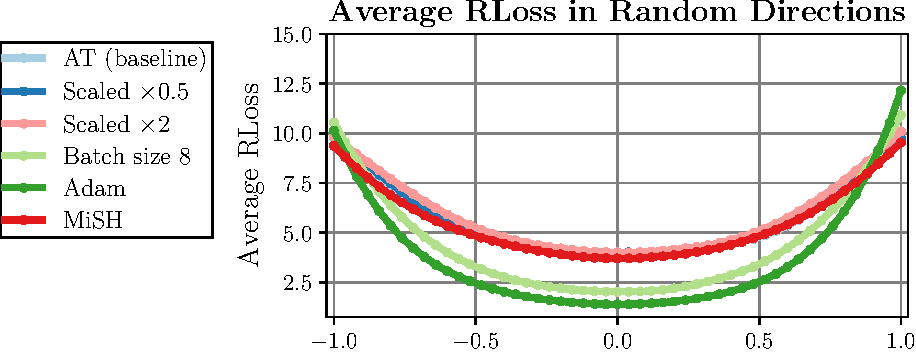
\includegraphics[width=0.425\textwidth]{plots_supp_random_filter}
	\vspace*{2px}
	
	\hspace*{-0.35cm}
	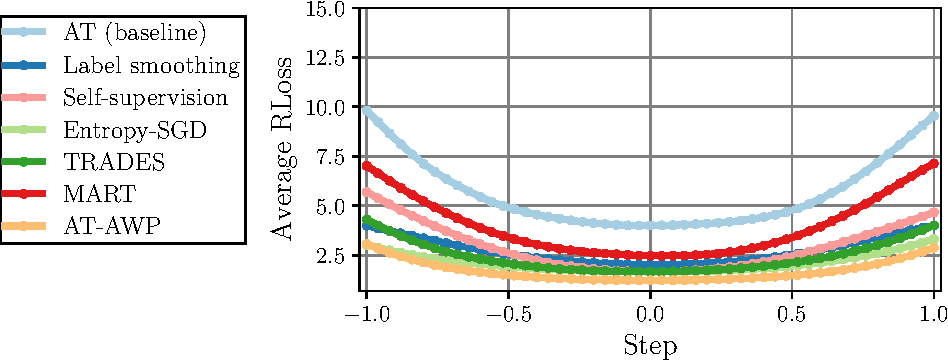
\includegraphics[width=0.44\textwidth]{plots_supp_random_filter2}
	\vspace*{-4px}
	\caption{\textbf{Filter-Wise Normalization:} Compared to the \RCE landscape visualizations in the main paper, using per-layer normalization in \eqnref{eq:supp-normalization}, we follow \cite{LiNIPS2018} and use filter-wise normalization in \eqnref{eq:supp-normalization-filter}. Again, we plot mean \RCE across $10$ random directions. However, this does not change results significantly, flatness remains difficult to judge and compare in an objective way. Filter-wise normalization, however, ``looks'' generally flatter.}
	\label{fig:supp-visualization-li}
	\vspace*{-6px}
\end{figure}

\section{Computing Flatness in \RCE}
\label{sec:supp-flatness-computation}

\begin{figure*}[t]
	\centering
	\vspace*{-0.2cm}
	\begin{minipage}[t]{0.31\textwidth}
		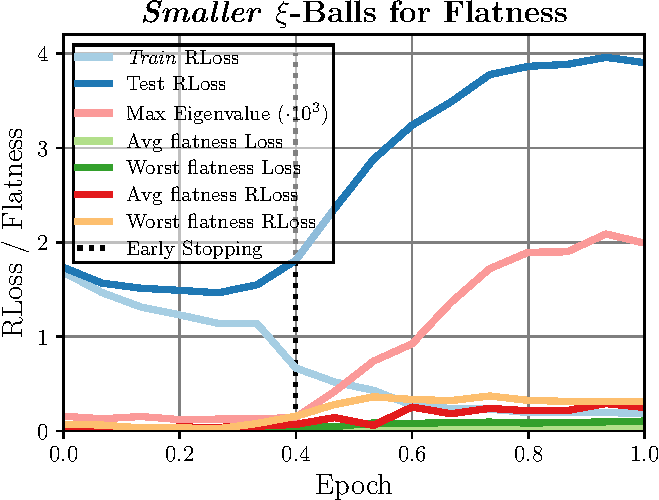
\includegraphics[width=\textwidth]{plots_supp_flatness_epochs_small}
	\end{minipage}
	\hspace*{2px}
	\begin{minipage}[t]{0.31\textwidth}
		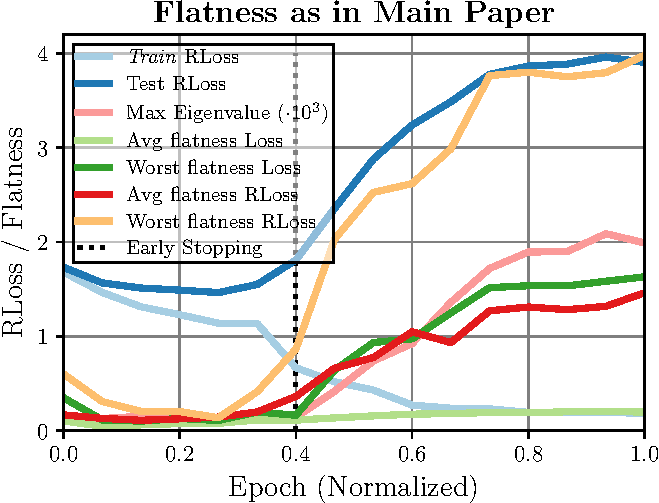
\includegraphics[width=\textwidth]{plots_supp_flatness_epochs}
	\end{minipage}
	\hspace*{2px}
	\begin{minipage}[t]{0.31\textwidth}
		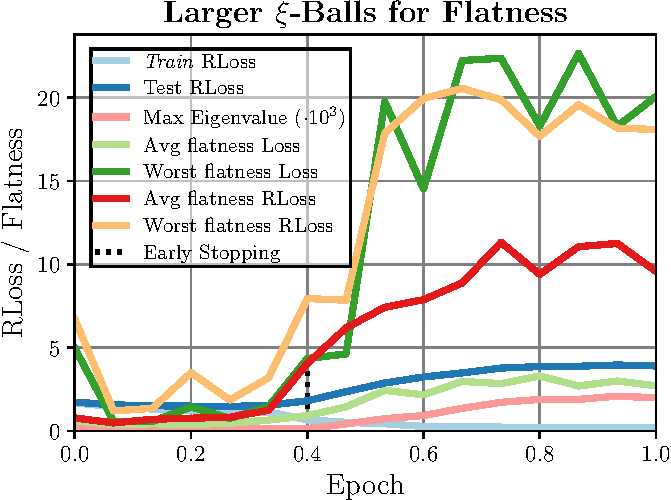
\includegraphics[width=\textwidth]{plots_supp_flatness_epochs_large}
	\end{minipage}
	\vspace*{-6px}
	\caption{\textbf{Flatness Throughout Training, Ablation:} We plot train and test \RCE, maximum Hessian eigenvalue $\lambda_{\text{max}}$, average-/worst-case flatness of (clean) \CE as well as average-/worst-case flatness on \RCE. We consider $\xi{=}0.25$/$\xi{=}0.001$ (left), $\xi{=}0.5$/$\xi{=}0.003$ (middle and main paper), and $\xi{=}0.75$/$\xi{=}0.005$ for average-/worst-case flatness, respectively. If the neighborhood $b_\xi(w)$ is chosen too small (left), increases/changes in flatness during robust overfitting are difficult to measure due to fluctuations throughout training. Chosen too large (right), in contrast, worst-case flatness (both in \CE and \RCE) quickly reaches unreasonably high loss values. This becomes problematic when comparing across models.}
	\label{fig:supp-flatness-epochs}
	\vspace*{-6px}
\end{figure*}

\textbf{Average-Case Flatness:}
%
The average-case flatness measure in \RCE is defined as:
\begin{align}
	\hspace*{-0.2cm}\begin{split}
		\mathbb{E}_{\nu}[\max\limits_{\|\delta\|_\infty \leq \epsilon} \mathcal{L}(f(x{+}\delta, w{+}\nu), y)]\text{\hphantom{aaaaaaa}}\\
		\text{\hphantom{aaaaaaa}}- \max\limits_{\|\delta\|_\infty \leq \epsilon} \mathcal{L}(f(x{+}\delta;w), y)
	\end{split}\label{eq:supp-average}
\end{align}
where $\mathbb{E}_{\nu}$ denotes the expectation over random weight perturbations $\nu \in B_\xi(w)$, $\mathcal{L}$ is the cross-entropy loss and $\max_{\|\delta\|_\infty \leq \epsilon}\mathcal{L}(f(x{+}\delta;w), y)$ represents the robust loss (\RCE). The first term is computed by randomly sampling $10$ weight perturbations from
\begin{align}
	B_\xi(w) = \{w + \nu : \|\nu^{(l)}\|_2 \leq \xi \|w^{(l)}\|_2 \forall\text{ layers }l\}.\label{eq:supp-ball}
\end{align}
For each weight perturbation $\nu$, the robust loss, defined as $\max_{\|\delta\|_\infty \leq \epsilon} \mathcal{L}(f(x{+}\delta, w{+}\nu), y)$, is estimated using PGD with $20$ iterations ($\epsilon = \nicefrac{8}{255}$, learning rate $0.007$ and signed gradient). This is done \emph{per-batch} (of size $128$) for the \emph{first} $1000$ test examples. Alternatively, the weights perturbations $\nu$ could also be fixed across batches (\ie, $10$ samples in total for $\lceil\nicefrac{1000}{128}\rceil$ batches). However, this is not possible for our worst-case flatness measure, as discussed next. Thus, for comparability, we sample random weight perturbations \emph{for each} batch individually. The second term is computed using PGD-$20$ with $10$ restarts, choosing the worst-case adversarial examples per test example (\ie, maximizing \RCE).

Sampling in $B_\xi(w)$ is accomplished by sampling individually per layer. That is, for each layer $l$, we compute $\xi' := \xi \cdot \|w^{(l)}\|_2$ given the original weights $w$. Then, a random vector $\nu^{(l)}$ with $\|\nu^{(l)}\|_2 \leq \xi'$ is sampled. This is done for each layer, handling weights and biases as separate layers, but ignoring batch normalization \cite{IoffeICML2015} parameters.

\textbf{Worst-Case Flatness:}
%
Worst-case flatness is defined as:
\begin{align}
	\begin{split}
		\max_{\nu \in B_\xi(w)} \max\limits_{\|\delta\|_\infty \leq \epsilon} &\mathcal{L}(f(x{+}\delta, w{+}\nu), y)\\
		&- \max\limits_{\|\delta\|_\infty \leq \epsilon} \mathcal{L}(f(x{+}\delta;w), y).
	\end{split}\label{eq:supp-worst}
\end{align}
Here, the expectation over $\nu$ in \eqnref{eq:supp-average} is replaced by a maximum over $\nu \in B_\xi(w)$, considering smaller $\xi$. In practice, the first term in \eqnref{eq:supp-worst} is computed by \emph{jointly} optimizing over weight perturbation $\nu$ and input perturbation(s) $\delta$ on a per-batch basis (of size $B = 128$). This means, after random initialization of $\delta_b$, $\forall b = 1,\ldots,B$, and $\nu \in B_\xi(w)$, each iteration computes and applies updates
\begin{align}
	\Delta_\nu = \nabla_\nu \sum_{b = 1}^B\mathcal{L}(f(x_b + \delta_b; w + \nu), y_b)\\
	\Delta_{\delta_b} = \nabla_{\delta_b} \sum_{b = 1}^B\mathcal{L}(f(x_b + \delta_b; w + \nu), y_b)
\end{align}
before projecting $\delta_b$ and $\nu$ onto the constraints $\|\delta_b\|_\infty \leq \epsilon$ and $\|\nu^{(l)}\|_2 \leq \xi \|w^{(l)}|_2$. The latter projection is applied in a per-layer basis, similar to sampling as described above. For the adversarial weight perturbation $\nu$, we use learning rate $0.001$, after normalizing the update $\Delta_\nu$ per-layer as in \eqnref{eq:supp-normalization}. We run $20$ iterations with $10$ restarts for each batch.

\textbf{Flatness of Clean Loss Landscape:}
%
We can also consider both \eqnref{eq:supp-average} and \eqnref{eq:supp-worst} on the \emph{clean} (cross-entropy) loss (``\CE''), \ie, $\mathcal{L}(f(x, w{+}\nu), y)$ instead of $\max_{\|\delta\|_\infty \leq \epsilon} \mathcal{L}(f(x{+}\delta, w{+}\nu), y)$. \red{We note that \RCE is an upper bound of (clean) \CE. Thus, flatness in \RCE and \CE are connected. However, Pearson correlation between \RCE and average-case flatness in (clean) \CE is only $0.27$, compared to $0.85$ for average-case flatness in \emph{\RCE}. This indicates that correctly measuring flatness in \RCE is crucial to empirically establish a relationship between robustness and flatness.}

\begin{figure*}[t]
	\centering
	\vspace*{-0.2cm}
	\hspace*{-1.75cm}
	\begin{minipage}[t]{0.28\textwidth}
		\vspace*{0px}
		
		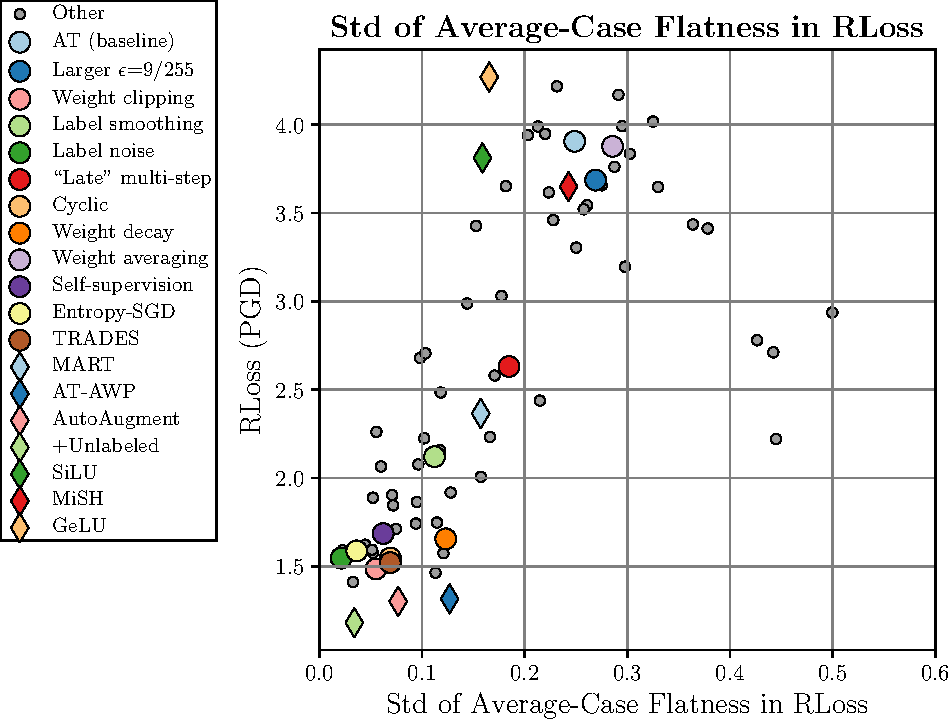
\includegraphics[height=3.5cm]{plots_supp_flatness_correlation_seq_loss_std}
	\end{minipage}
	\begin{minipage}[t]{0.2\textwidth}
		\vspace*{0px}
		
		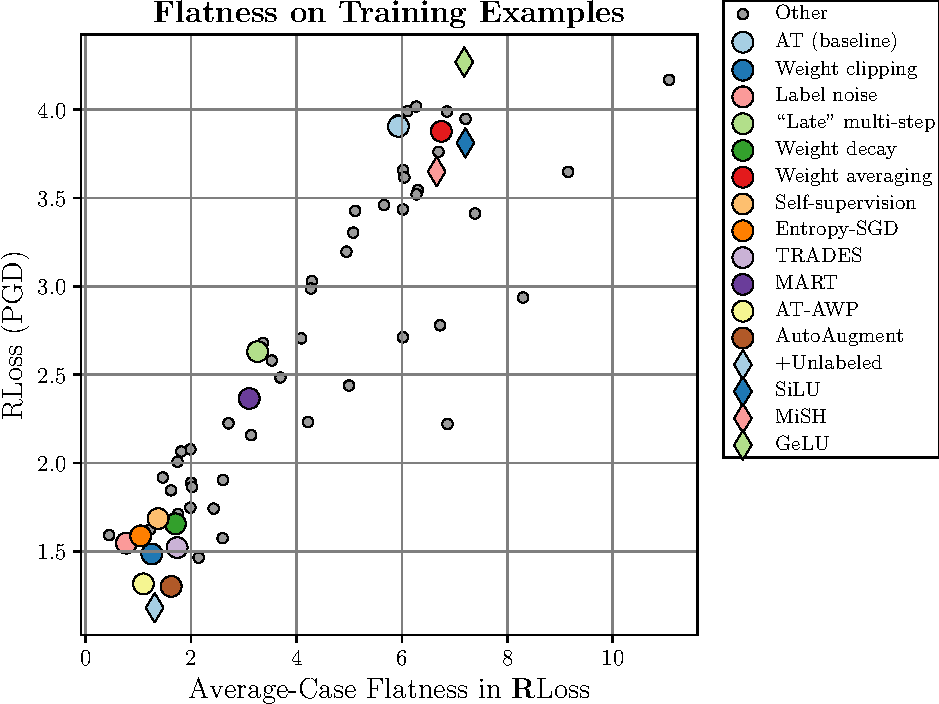
\includegraphics[height=3.5cm]{plots_supp_flatness_correlation_seq_train_loss}
	\end{minipage}
	\begin{minipage}[t]{0.2\textwidth}
		\vspace*{0px}
		
		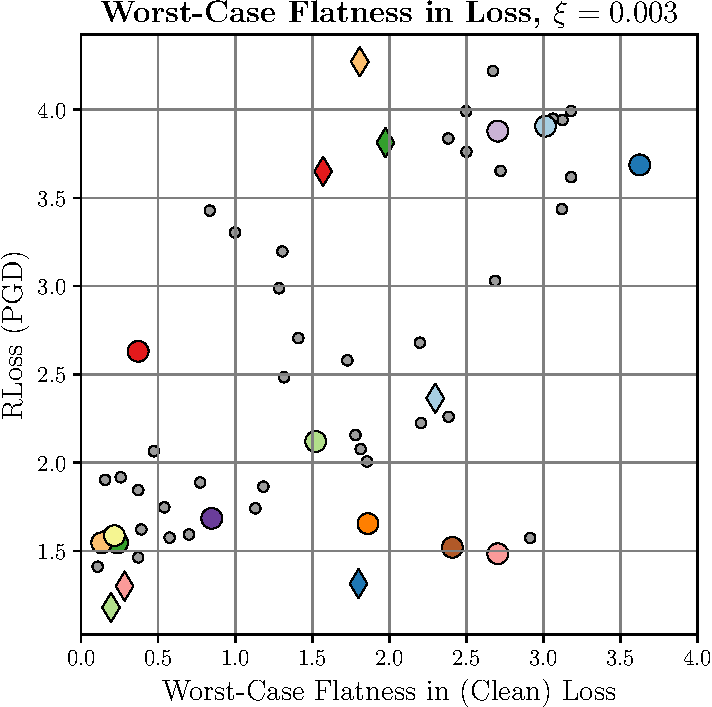
\includegraphics[height=3.5cm]{plots_supp_flatness_correlation_adv_loss_e0003}
	\end{minipage}
	\begin{minipage}[t]{0.25\textwidth}
			\vspace*{0px}
			
			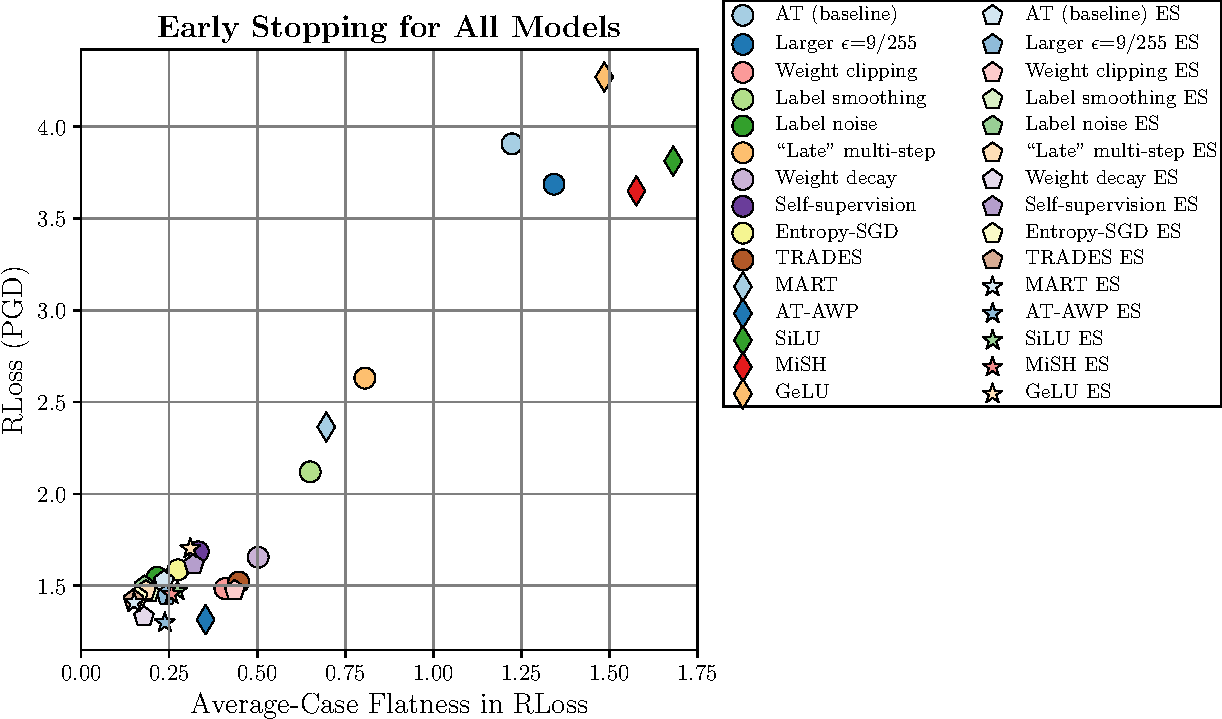
\includegraphics[height=3.5cm]{plots_supp_flatness_seq_early_stopping_all}
			
			\begin{tikzpicture}[overlay,remember picture]
				\node[anchor=south west] at (1.8,0.75){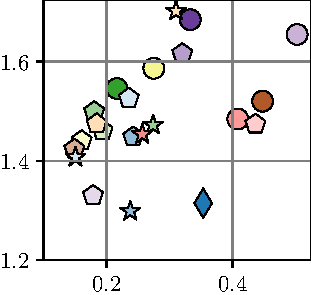
\includegraphics[height=1.4cm]{plots_supp_flatness_seq_early_stopping_zoom}};
			\end{tikzpicture}
		\end{minipage}
	\vspace*{-18px}
	\caption{\textbf{Left: Standard Deviation of Average-Case Flatness:} We plot \RCE (y-axis) against the standard deviation (std) in our average-case flatness measure (x-axis). Note that the standard-deviation is due to the random weight perturbations $\nu$ in \eqnref{eq:supp-average}. Interestingly, more robust methods are not only flatter, but our average-case flatness measure also has lower standard deviation. \textbf{Middle Left: Average-Case Flatness of Train \RCE:} \emph{Test} \RCE plotted against our average-case flatness measure as computed on \emph{training} examples. Even on the training set, flatness is predictive of robust generalization, \ie, adversarial robustness on the test set. The relationship, however, is weaker compared to average-case flatness on test examples. \textbf{Middle Right: Worst-Case Flatness in (Clean) \CE:} As worst-case flatness in the \emph{clean} \CE landscape also mirrors robust overfitting in \figref{fig:supp-flatness-epochs}, we plot \RCE against worst-case flatness in \CE. Even though flatness is measured considering clean \CE, many methods improving robustness (\ie, lower \RCE) exhibit surprisingly good flatness. \textbf{Right: Early Stopping for all Models:} \RCE vs\onedot average-case flatness for all models where early stopping improves adversarial robustness. For example, this is not the case for AutoAugment or AT with unlabeled examples. Across all models, early stopping improves both robustness and flatness. For clarity we provide a zoomed-in plot for the lower left corner.}
	\label{fig:supp-flatness-misc}
\end{figure*}

\subsection{Ablation for Flatness Measures}
\label{sec:supp-flatness-ablation}
 
\textbf{Flatness Throughout Training:}
%
\figref{fig:supp-flatness-epochs} shows average- and worst-case flatness on both clean as well as robust loss (\CE and \RCE) throughout training of our AT baseline. We consider different sizes of the neighborhood $B_\xi(w)$ for computing our flatness measures: $\xi{=}0.25$/$\xi{=}0.001$ (left), $\xi{=}0.5$/$\xi{=}0.003$ (middle, as in main paper), and $\xi{=}0.75$/$\xi{=}0.005$ for average-/worst-case flatness, respectively. While average-case flatness of \emph{clean} \CE does \emph{not} mirror robust overfitting very well, its worst-case pendant increases during overfitting, even though \RCE is \emph{not} taken into account. Furthermore, if the neighborhood $B_\xi(w)$ is chosen too small, the flatness measures are not sensitive enough to be discriminative (\cf left). \figref{fig:supp-flatness-epochs} also shows that, throughout training of one model, the largest Hessian eigenvalue mirrors robust overfitting. Overall, this means that early stopping essentially improves adversarial robustness by finding flatter minima. This is confirmed in \figref{fig:supp-flatness-misc} (right), showing that early stopping consistently improves robustness and flatness.

\textbf{Standard Deviation in Average-Case Flatness:} 
%
In \figref{fig:supp-flatness-misc} (left), the x-axis plots the standard deviation in our average-case flatness measure (in \RCE). Note that the standard deviation originates in the random samples $\nu$ used to calculate \eqnref{eq:supp-average}. First of all, standard deviation tends to be small (\ie, $\leq 0.3$) across almost all models. This means that our findings in the main paper, \ie, the strong correlation between flatness and \RCE, is supported by low standard deviation. More importantly, the standard deviation \emph{reduces} for particularly robust methods.

\textbf{Average-Case Flatness on Training Examples:}
%
\figref{fig:supp-flatness-misc} (middle left) shows that average-case flatness in \RCE is also predictive for robust generalization when computed on \emph{training} examples. However, the correlation between (test) \RCE and (train) flatness is less clear, \ie, there is a larger ``spread'' across methods. Here, we use the first $1000$ training examples to compute average-case flatness.

\textbf{Worst-Case Flatness on \emph{Clean} \CE:}
%
In \figref{fig:supp-flatness-epochs}, worst-case flatness on clean \CE also correlates with robust overfitting. Thus, in \figref{fig:supp-flatness-misc} (middle right), we plot \RCE against worst-case flatness of \CE, showing that there is no clear relationship across models. Nevertheless, many methods improving adversarial robustness also result in flatter minima in the clean loss landscape. This is sensible as \RCE is generally an upper bound for (clean) \CE. On the other hand, flatness in \CE is \emph{not} discriminative enough to clearly distinguish between robust and less robust models.

\begin{figure*}[t]
	\centering
	\vspace*{-0.2cm}
	\begin{minipage}[t]{0.3\textwidth}
		\vspace*{0px}
		
		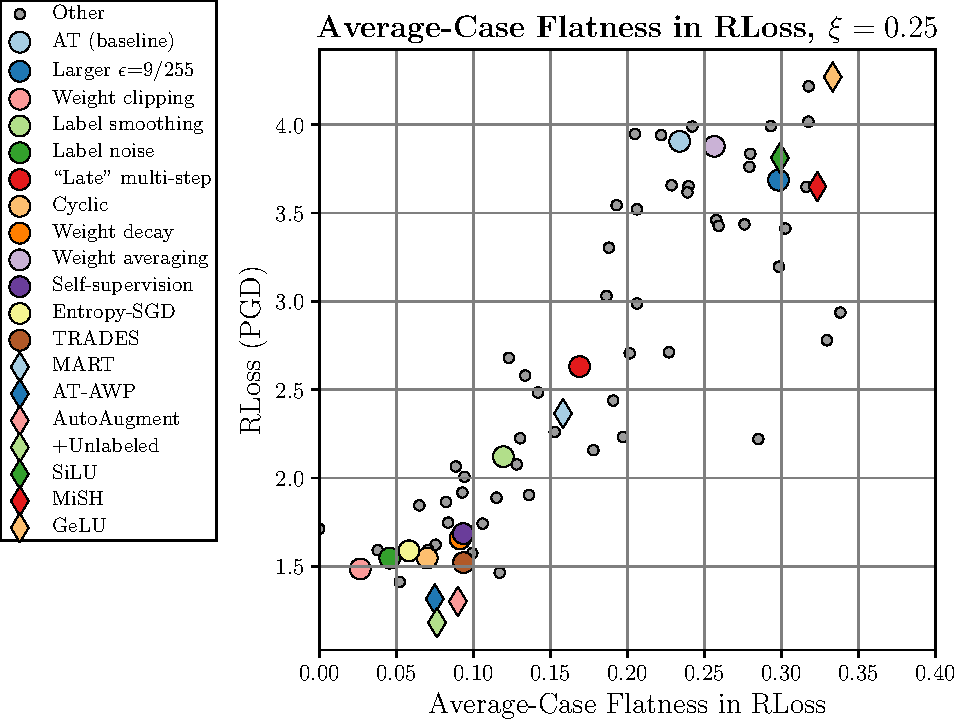
\includegraphics[height=3.6cm]{plots_supp_flatness_correlation_seq_loss_e025}
	\end{minipage}
	\begin{minipage}[t]{0.22\textwidth}
		\vspace*{0px}
		
		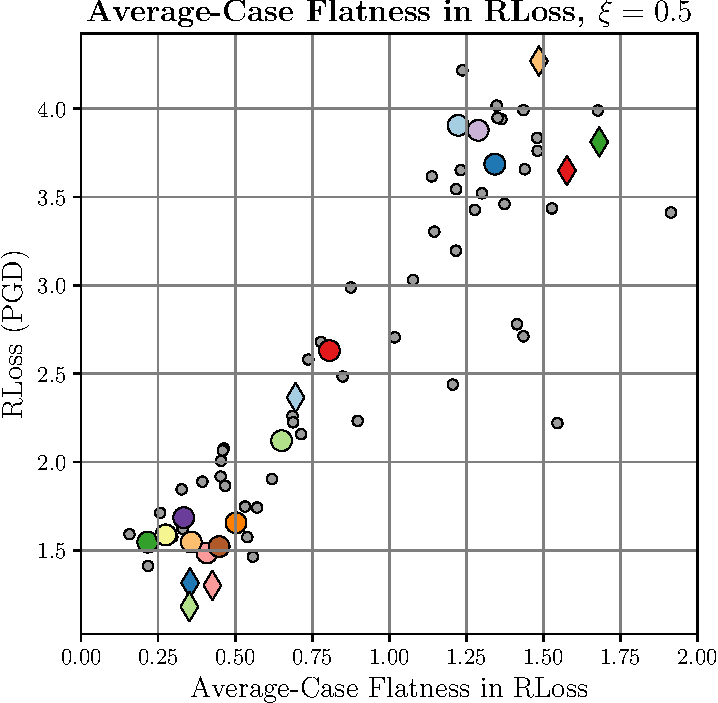
\includegraphics[height=3.6cm]{plots_supp_flatness_correlation_seq_loss_e05}
	\end{minipage}
	\begin{minipage}[t]{0.22\textwidth}
		\vspace*{0px}
		
		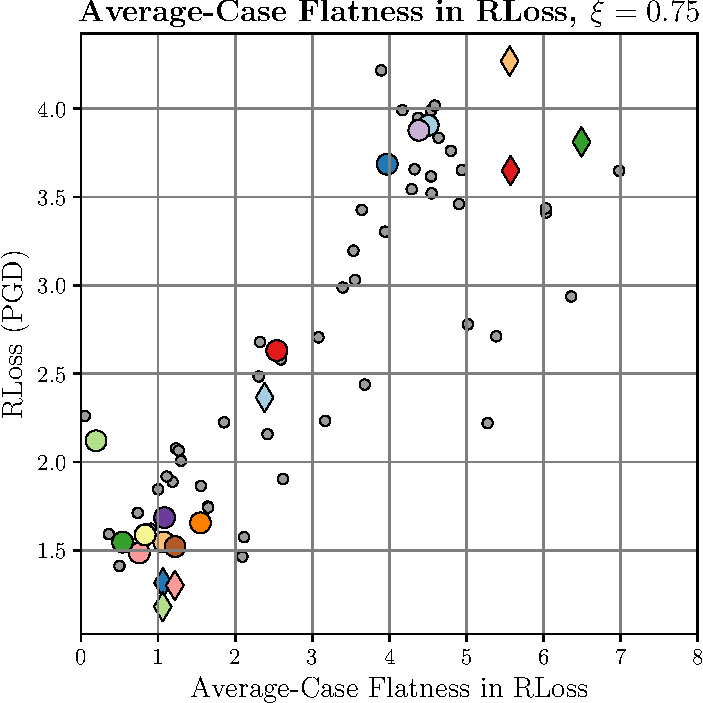
\includegraphics[height=3.6cm]{plots_supp_flatness_correlation_seq_loss_e075}
	\end{minipage}
	\begin{minipage}[t]{0.22\textwidth}
		\vspace*{0px}
		
		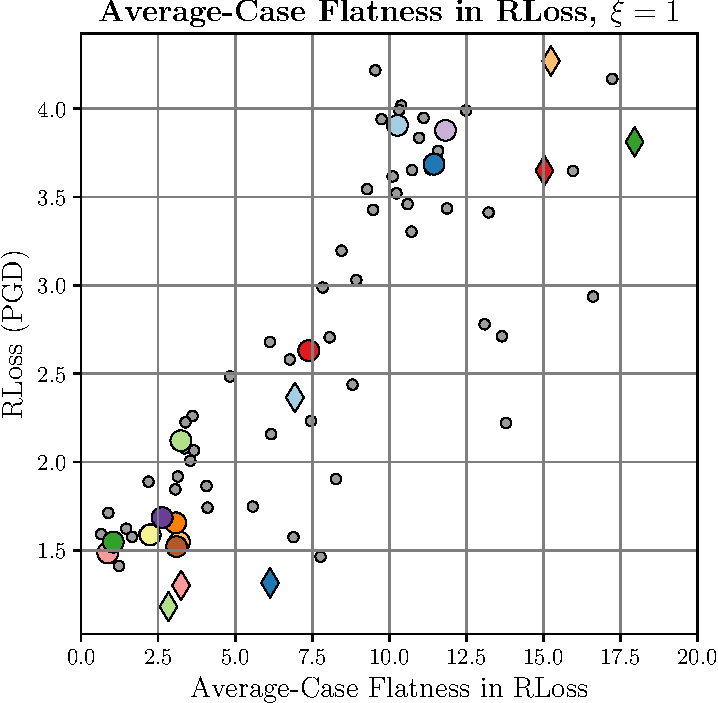
\includegraphics[height=3.6cm]{plots_supp_flatness_correlation_seq_loss_e1}
	\end{minipage}
	\\[6px]
	
	{\color{black!75}\rule{\textwidth}{0.65px}}
	\\[-6px]
	
	\begin{minipage}[t]{0.3\textwidth}
		\vspace*{0px}
		
		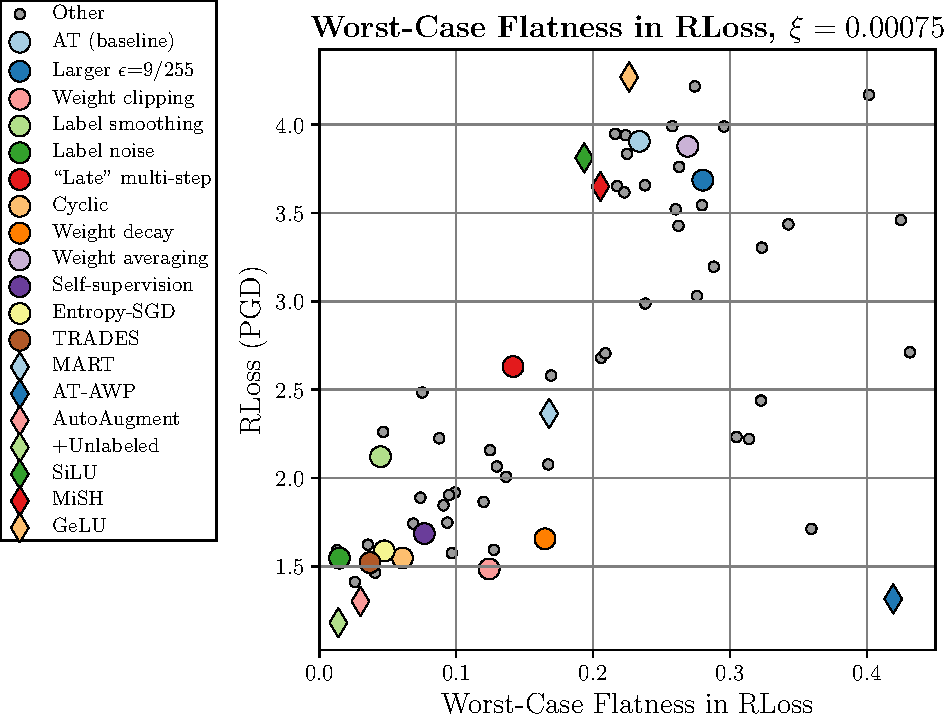
\includegraphics[height=3.6cm]{plots_supp_flatness_correlation_joint_loss_e000075}
	\end{minipage}
	\begin{minipage}[t]{0.22\textwidth}
		\vspace*{0px}
		
		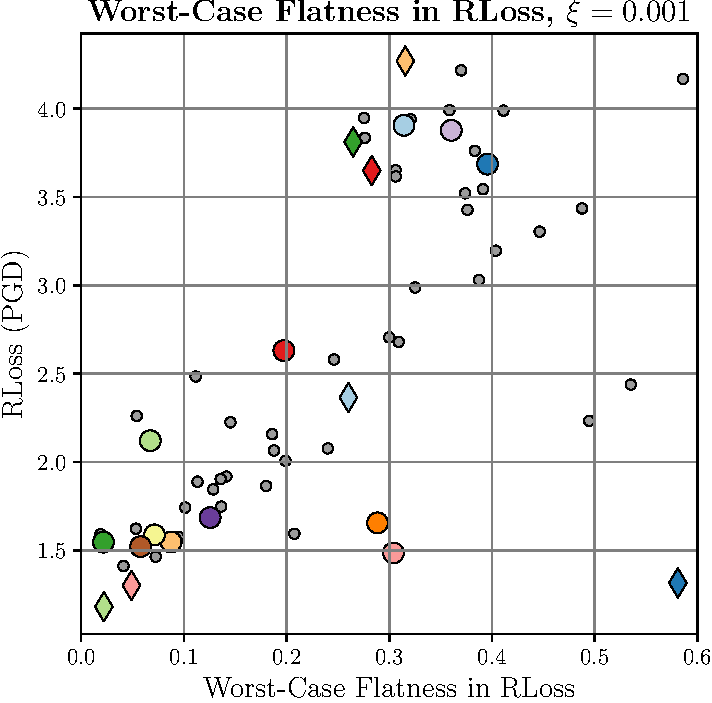
\includegraphics[height=3.6cm]{plots_supp_flatness_correlation_joint_loss_e0001}
	\end{minipage}
	\begin{minipage}[t]{0.22\textwidth}
		\vspace*{0px}
		
		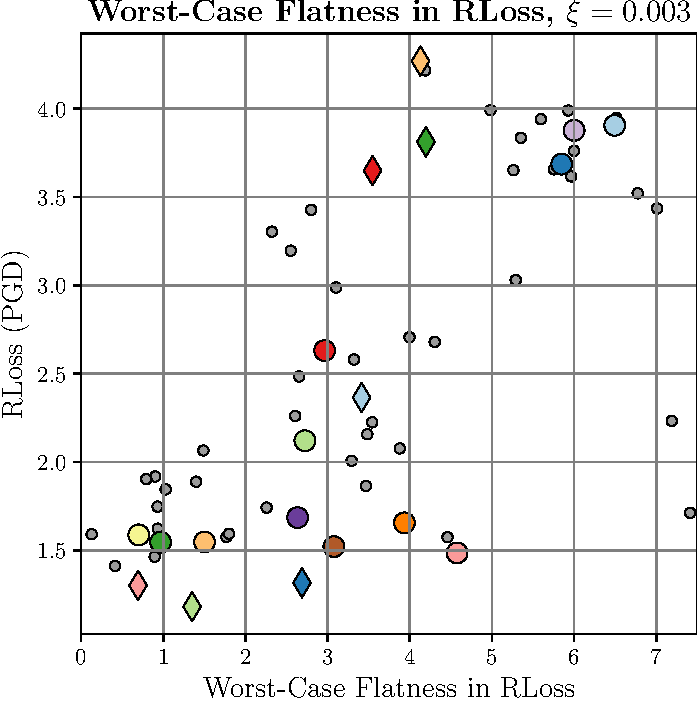
\includegraphics[height=3.6cm]{plots_supp_flatness_correlation_joint_loss_e0003}
	\end{minipage}
	\begin{minipage}[t]{0.22\textwidth}
		\vspace*{0px}
		
		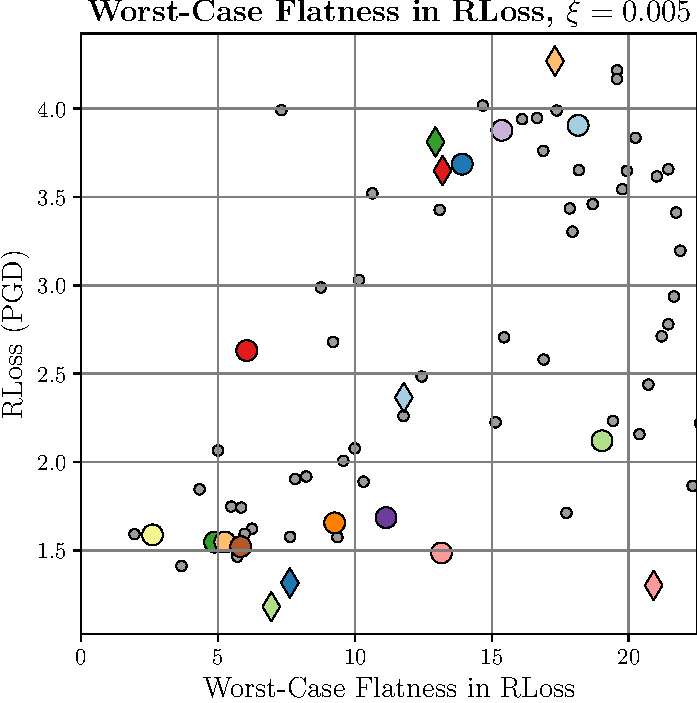
\includegraphics[height=3.6cm]{plots_supp_flatness_correlation_joint_loss_e0005}
	\end{minipage}
	\caption{\textbf{Flatness in \RCE, Ablation for $B_\xi(w)$:} \RCE(y-axis) plotted against average-case (top) and worst-case (bottom) flatness in \RCE (x-axis).
	\textbf{Top:} We consider $\xi \in \{0.25, 0.5, 0.75, 1\}$ for average-case flatness. The clear relationship between adversarial robustness, \ie, low \RCE, and flatness shown for $\xi = 0.5$ in the main paper can be reproduced for all cases. \textbf{Bottom:} For worst-case flatness, we consider $\xi \in \{0.00075, 0.001, 0.003, 0.005\}$. When chosen too large, \eg, $\xi = 0.005$, however, variance seems to increase, making the relationship less clear. For small $\xi$, \eg, $\xi = 0.00075$, the correlation between robustness and flatness is pronounced, except for a few outliers, including AT-AWP \cite{WuNIPS2020}.}
	\label{fig:supp-flatness-ablation}
\end{figure*}

\textbf{Ablation for $B_\xi(w)$:}
%
For computing our average- and worst-case flatness measures (in \RCE), we considered various sizes of neighborhoods in weight space, \ie $B_\xi(w)$ from \eqnref{eq:supp-ball} for different $\xi$. \figref{fig:supp-flatness-ablation} considers $\xi \in \{0.25, 0.5, 0.75, 1\}$ for average-case flatness (top) and $\xi \in \{0.00075, 0.001, 0.003, 0.005\}$ for worst-case flatness (bottom). In both cases, we plot \RCE (y-axis) against flatness in \RCE (y-axis), as known from the main paper. Average-case flatness using small $\xi = 0.25$ results in significantly smaller values, between $0$ and $0.4$, \ie, the increase in \RCE in random weight directions is rather small. Still, the relationship between adversarial robustness and flatness is clearly visible. The same holds for larger $\xi \in \{0.75, 1\}$. Worst-case flatness generally gives a less clear picture regarding the relationship between robustness and flatness.
Additionally, for larger $\xi \in \{0.003, 0.005\}$, variance seems to increase such that this relationship becomes less pronounced. In contrast to average-case flatness, the variance is not induced by the $10$ restarts used for \eqnref{eq:supp-worst}, but caused by training itself. Indeed, re-training our AT baseline leads to a worst-case flatness in \RCE of $5.1$, a significant reduction from $6.49$ as obtained for our original baseline. Overall, however, the observations from the main paper can be confirmed using different sizes of the neighborhood $B_\xi(w)$.

\section{Scaling Networks and Scale-Invariance}
\label{sec:supp-scaling}

\textbf{Scale-Invariance:}
%
In the main paper, we presented a simple experiment to show that our measures of flatness in \RCE are scale-invariant: we scaled weights \emph{and} biases of \emph{all} convolutional layers in our adversarially trained ResNet-18 \cite{HeCVPR2016} by factor $s \in \{0.5, 2\}$. Note that all convolutional layers in the ResNet are followed by batch normalization layers \cite{IoffeICML2015}. Thus, the effect of scaling is essentially ``canceled out'', \ie, these convolutional layers are scale-invariant. Thus, the prediction stays roughly constant. \figref{fig:supp-scaling} (left) shows \RCE landscape visualizations for AT and its scaled variants in random and adversarial weight directions. Clearly, scaling AT has negligible impact on the \RCE landscape in both cases. \figref{fig:supp-scaling} (right) shows that our flatness measures remain invariant, as well. As $B_\xi(w)$ in \eqnref{eq:supp-ball} is defined \emph{per-layer} (weights and biases separately) and \emph{relative} to $w$, the neighborhood increases alongside the weights, rendering visualization and flatness measures invariant.
\red{When, for example, scaling up specific layers and scaling down others, as discussed in \cite{DinhICML2017}, causes the neighborhood $B_\xi(w)$ to increase or decrease in size for these particular layers. Thus, following \cite{DinhICML2017}, scaling up the first layer of a two-layer ReLU network by $\alpha$ and scaling down the second layer by $\nicefrac{1}{\alpha}$ (keeping the output constant), has no effect in terms of measuring flatness as the per-layer neighborhood $B_\xi(w)$ is scaled accordingly, as well.}
The Hessian eigenspectrum, in contrast, scales with the models, \cf \tabref{tab:supp-convexity}, and is not suited to quantify flatness.

\textbf{Convexity and Flatness:}
%
\tabref{tab:supp-convexity} also presents the convexity metric introduced in \cite{LiNIPS2018}: $\nicefrac{|\lambda_{\text{min}}|}{|\lambda_{\text{max}}|}$ with $\lambda_{\text{min/max}}$ being largest/smallest Hessian eigenvalue. Note that the Hessian is computed following \cite{LiNIPS2018} \wrt to the \emph{clean} (cross-entropy) loss, not taking into account adversarial examples. The intuition is that negative eigenvalues with large absolute value correspond to non-convex directions in weight space. If these eigenvalues are large in relation to the positive eigenvalues, there is assumed to be significant non-convexity ``around'' the found minimum. \tabref{tab:supp-convexity} shows that this fraction is usually very small, as also found in \cite{LiNIPS2018}. However, \tabref{tab:supp-convexity} also shows that this convexity measure is not clearly correlated with adversarial robustness.

\section{Detailed Experimental Setup}
\label{sec:supp-setup}

We focus our experiments on \CifarT \cite{Krizhevsky2009}, consisting of $50\text{k}$ training examples and $10\text{k}$ test examples of size $32\times32$ (in color) and $K = 10$ class labels. We use all training examples during training, but withhold the \emph{last} $500$ test examples for early stopping. Evaluation is performed on the \emph{first} $1000$ test examples, due to long runtimes of AutoAttack \cite{CroceARXIV2020} and our flatness measures (on \RCE). Any evaluation on the training set is performed on the first $1000$ training examples (\eg, in \figref{fig:supp-flatness-misc}, middle).

\begin{figure*}[t]
	\centering
	\vspace*{-0.2cm}
	\begin{minipage}[t]{0.26\textwidth}
		\vspace*{0px}
		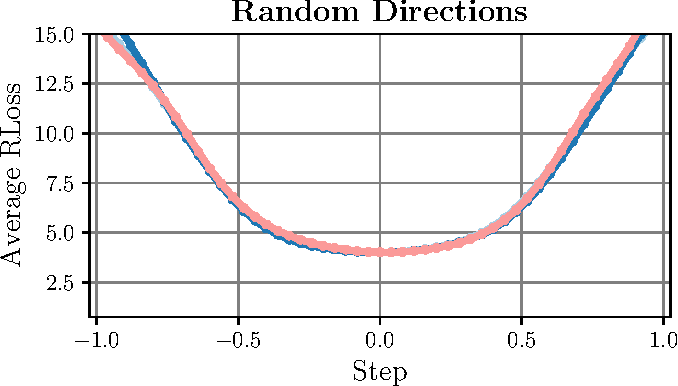
\includegraphics[width=\textwidth]{plots_supp_scaling_random}
	\end{minipage}
	\begin{minipage}[t]{0.155\textwidth}
		\vspace*{0px}
		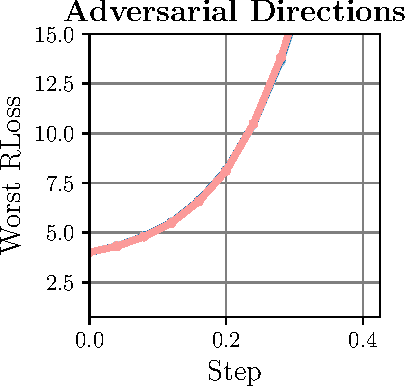
\includegraphics[width=\textwidth]{plots_supp_scaling_adversarial}
	\end{minipage}
	\hspace*{0.25cm}
	\begin{minipage}[t]{0.38\textwidth}
		\vspace*{0px}
		\scriptsize
		{
			\setlength{\tabcolsep}{0pt}
		    \newcolumntype{C}[1]{@{}>{\centering\arraybackslash}p{#1}@{}}
			\begin{tabularx}{\textwidth}{|X|C{0.85cm}|C{1.5cm}|C{0.85cm}|C{0.85cm}|C{0.85cm}|}
				\hline
				\hspace*{2px} Model & \multicolumn{2}{c|}{\bfseries Robustness} & \multicolumn{3}{c|}{\bfseries Flatness}\\
				\hline
				& \RTE $\downarrow$ & \RTE $\downarrow$ & Worst & Avg & Worst\\
				& (test) & (train) & \emph{Loss} & \textbf{RLoss} & \textbf{RLoss}\\
				\hline
				\hline		
				\hspace*{2px} Scaled $\times0.5$ & 60.9 & 8.4 (-52.5) &  0.86 & 1.36 & 6.50\\
				\hspace*{2px} AT (baseline) & 61.0 & 8.4 (-52.6) & 0.86 & 1.21 & 6.48\\
				\hspace*{2px} Scaled $\times2$ & 61.0 & 8.3 (-52.7) & 0.86 & 1.27 & 6.49\\
				\hline
			\end{tabularx}
		}
	\end{minipage}
	\vspace*{-6px}
	\caption{\textbf{Flatness and Scale-Invariance.} \textbf{Left:} We plot average \RCE and worst \RCE along random and adversarial directions, as discussed in \secref{sec:supp-visualization}, for AT and its scaled variants, $\times0.5$ and $\times2$. Clearly, \RCE landscape looks nearly identical. \textbf{Right:} Robustness against PGD-$20$ on train and test examples, as well as average- and worst-case flatness measures on \RCE. For completeness, we also include worst-case flatness on clean \CE. All of these measures are nearly invariant to scaling. The shown differences can be attributed to randomness in computing these measures.}
	\label{fig:supp-scaling}

\end{figure*}

As network architecture, we use ResNet-18 \cite{HeCVPR2016} with batch normalization \cite{IoffeICML2015} and ReLU activations. Our AT baseline (\ie, default model) is trained using SGD for $150$ epochs, batch size $128$, learning rate $0.05$, reduced by factor $0.1$ at $60$, $90$ and $120$ epochs, weight decay $0.005$ and momentum $0.9$. We save snapshots every $5$ epochs to perform early stopping, but do \emph{not} use early stopping by default. We whiten input examples by subtracting the (per-channel) mean and dividing by standard deviation. We use standard data augmentation, considering random flips and cropping (by up to $4$ pixels per side). By default, we use $7$ iterations PGD, with learning rate $0.007$, signed gradient and $\epsilon = \nicefrac{8}{255}$ to compute $L_\infty$ adversarial examples. Note that no momentum \cite{DongCVPR2018} or backtracking \cite{StutzICML2020} is used for PGD. The training curves in \figref{fig:supp-training-curves} correspond to robustness measured using the $7$-iterations PGD attack used for training, which we also use for early stopping (with $5$ random restarts).

For evaluation, we run PGD for $20$ iterations and $10$ random restarts, taking the worst-case adversarial example per test example \cite{StutzICML2020}. Our results considering robust loss (\RCE) are based on PGD, while we report robust test error (\RTE) using AutoAttack \cite{CroceARXIV2020}. \red{Note that AutoAttack does \emph{not} maximize cross-entropy loss as it stops when adversarial examples are found. Thus, it is not suitable to estimate \RCE.} Robust test error is calculated as the fraction of test examples that are either mis-classified or successfully attacked. The distinction between PGD-$20$ and AutoAttack is important as AutoAttack does \emph{not} maximize cross-entropy loss, resulting in an under-estimation of \RCE, while PGD-$20$ generally underestimates \RTE. Computation of our average- and worst-case flatness measure is detailed in \secref{sec:supp-flatness-computation}.

Everything is implemented in PyTorch~\cite{PaszkeNIPSWORK2017}.

\section{Methods}
\label{sec:supp-methods}

In the following, we briefly elaborate on the individual methods considered in our experiments.

\textbf{Learning Rate Schedules:}
%
Besides our default, multi-step learning rate schedule (learning rate $0.05$, reduced by factor $0.1$ after epochs $60$, $90$, and $120$), we followed \cite{PangARXIV2020b} and implemented the following learning rate schedules: First, simply using a constant learning rate of $0.05$. Second, only two ``late'' learning rate reductions at epochs $140$ and $145$, as done in \cite{QinNIPS2019}. Third, using a cyclic learning rate, interpolating between a learning rate of $0.2$ and $0$ for $30$ epochs per cycle, as, \eg, done in \cite{WongARXIV2020}. We consider training for up to $4$ cycles ($=120$ epochs). These learning rate schedules are available as part of PyTorch \cite{PaszkeNIPSWORK2017}.

\textbf{Label Smoothing:}
%
In \cite{SzegedyCVPR2016}, label smoothing is introduced as regularization to improve (clean) generalization by \emph{not} enforcing one-hot labels in the cross-entropy loss. Instead, for label $y$ and $K = 10$ classes, a target distribution $p \in [0,1]^K$ (subject to $\sum_i p_i = 1$) with $p_y = 1 - \tau$ (correct label) and $p_i = \nicefrac{\tau}{K - 1}$ for $i \neq y$ (all other labels) is enforced. During AT, we only apply label smoothing for the weight update, not for PGD. We consider $\tau \in \{0.1, 0.2, 0.3\}$.

\textbf{Label Noise:}
%
Instead of explicitly enforcing a ``smoothed'' target distribution, we also consider injecting label noise during training. In each batch, we sample random labels for a fraction of $\tau$ of the examples. Note that the labels are sampled uniformly across all $K = 10$ classes. Thus, in expectation, the enforced target distribution is $p_y = 1 - \tau + \nicefrac{\tau}{K}$ and $p_i = \nicefrac{\tau - \nicefrac{\tau}{K}}{K - 1}$. As result, this is equivalent to label smoothing with $\tau = \tau - \nicefrac{\tau}{K}$. In contrast to label smoothing, this distribution is not enforced explicitly in the cross-entropy loss. As above, adversarial examples are computed against the true labels (without label noise) and label noise is injected for the weight update. We consider $\tau \in \{0.1, 0.2, 0.3, 0.4, 0.5\}$. While label smoothing does not further improve adversarial robustness for $\tau > 0.3$, label noise proved very effective in avoiding robust overfitting, which is why we also consider $\tau = 0.4$ or $0.5$.

\textbf{Weight Averaging:}
%
To implement weight averaging \cite{IzmailovUAI2018}, we follow \cite{GowalARXIV2020} and keep a ``running'' average $\bar{w}$ of the model's weights throughout training, updated in each iteration $t$ as follows: 
\begin{align}
	\bar{w}^{(t)} = \tau \bar{w}^{(t - 1)} + (1 - \tau) w^{(t)}
\end{align}
where $w^{(t)}$ are the weights in iteration $t$ \emph{after} the gradient update. Weight averaging is motivated by finding the weights $\bar{w}$ in the center of the found local minimum. As, depending on the learning rate, training tends to oscillate, the average of the iterates is assumed to be close to the actual center of the minimum. In our experiments, we consider $\tau \in \{0.98, 0.985, 0.99, 0.9975\}$.

\textbf{Weight Clipping:}
%
Following \cite{StutzMLSYS2021}, we implement weight clipping by clipping the weights to $[-w_{\text{max}}, w_{\text{max}}]$ after each training iteration. We found that $w_{\text{max}}$ can be chosen as small as $0.005$, which we found to work particularly well. Larger $w_{\text{max}}$ does \emph{not} have significant impact on adversarial robustness for AT. \cite{StutzMLSYS2021} argues that weight clipping together with minimizing cross-entropy loss leads to more redundant weights, improving robustness to random weight perturbations. As result, we also expect weight clipping to improve flatness. We consider $w_{\text{max}} \in \{0.005, 0.01, 0.025\}$.

\textbf{Ignoring Incorrect Examples \& Preventing Label Leaking:}
%
As robust overfitting in AT leads to large \RCE on incorrectly classified test examples, we investigate whether (a) \emph{not} computing adversarial examples on incorrectly classified examples (during training) or (b) computing adversarial examples against the predicted (not true) label (during training) helps to mitigate robust overfitting. These changes can be interpreted as ablations of MART \cite{WangICLR2020} and are easily implemented. Note that option (b) is essentially computing adversarial examples without label leaking \cite{KurakinARXIV2016}. However, as shown in \figref{fig:supp-ii-pll}, these two variants of AT have little to no impact on robust overfitting.

\begin{table}[t]
	\centering
	\vspace*{-0.2cm}
	\scriptsize
	\begin{tabularx}{0.475\textwidth}{|X|@{\hspace*{3px}}c@{\hspace*{3px}}|@{\hspace*{3px}}c@{\hspace*{3px}}|@{\hspace*{3px}}c@{\hspace*{3px}}|}
		\hline
		Model (\RTE against AutoAttack \cite{CroceICML2020}) & \RTE $\downarrow$ & $\lambda_{\text{max}}$ & $\frac{|\lambda_{\text{min}}|}{|\lambda_{\text{max}}|}$\\
		\hline
		\hline
		AT (baseline) & 62.8 & 1990 & 0.088\\
		Scaled $\times0.5$ & 62.8 & 7936 & 0.088\\
		Scaled $\times2$ & 62.8 & 505 & 0.088\\
		\hline
		Batch size $8$ & 58.2 & 3132 & 0.027\\
		Adam & 57.5 & 540 & 0.047\\
		\hline
		Label smoothing & 61.2 & 2484 & 0.085\\
		Self-supervision & 57.1 & 389 & 0.041\\
		Entropy-SGD & 58.6 & 5773 & 0.054\\
		TRADES & 56.7 & 947 & 0.089\\
		MART & 61 & 1285 & 0.087\\
		AT-AWP & 54.3 & 1200 & 0.241\\
		\hline
	\end{tabularx}
	\vspace*{-6px}
	\caption{\textbf{Hessian Eigenvalue $\lambda_{\text{max}}$ and Convexity:} For the models from \figref{fig:supp-visualization} and \ref{fig:supp-visualization-li}, we report \RTE against AutoAttack \cite{CroceARXIV2020}, the maximum Hessian eigenvalue $\lambda_{\text{max}}$ and the convexity measure of \cite{LiNIPS2018} computed as $\nicefrac{|\lambda_{\text{min}}|}{|\lambda_{\text{max}}|}$. This fraction is supposed to quantify the degree of non-convexity around the found minimum. As can be seen, neither $\lambda_{\text{max}}$ nor convexity correlate well with adversarial robustness. Regarding $\lambda_{\text{max}}$ this is due to the Hessian eigenspectrum not being scale-invariant, as shown for scaled versions ($\times0.5$ and $\times2$) of our AT baseline.}
	\label{tab:supp-convexity}
	\vspace*{-6px}
\end{table}

\textbf{AutoAugment:}
%
In \cite{CubukARXIV2018}, an automatic procedure for finding data augmentation policies is proposed, so-called AutoAugment. We use the found \CifarT policy (\cf \cite{CubukARXIV2018}, appendix), which includes quite extreme augmentations. For example, large translations are possible, rendering the image nearly completely uniform, only leaving few pixels at the border. In practice, AutoAugment usually prevents convergence and, thus, avoids overfitting. We further combine AutoAugment with CutOut \cite{DevriesARXIV2017} (using random $16\times 16$ ``cutouts''). We apply both AutoAugment and CutOut on top of our standard data augmentation, \ie, random flipping and cropping. We use publicly available PyTorch implementations\footnote{\url{https://github.com/DeepVoltaire/AutoAugment}, \url{https://github.com/uoguelph-mlrg/Cutout}}.

\textbf{Entropy-SGD}
%
\cite{ChaudhariICLR2017} explicitly encourages flatter minima by taking the so-called ``local'' entropy into account. As a result, Entropy-SGD not only finds ``deep'' minima (\ie, low loss values) but also flat ones. In practice, this is done using nested SGD: the inner loop approximates the local entropy using stochastic gradient Langevin dynamics (SGLD), the outer loop updates the weights. The number of inner iterations is denoted by $L$. While the original work \cite{ChaudhariICLR2017} uses $L$ in $[5, 20]$ on \CifarT, we experiment with $L \in \{1, 2, 3, 5\}$. Note that, for fair comparison, we train for $\nicefrac{150}{L}$ epochs.
For details on the Entropy-SGD algorithm, we refer to \cite{ChaudhariICLR2017}. Our implementation follows the official PyTorch implementation\footnote{\url{https://github.com/ucla-vision/entropy-sgd}}.

\begin{figure}[t]
	\centering
	\vspace*{-0.2cm}
	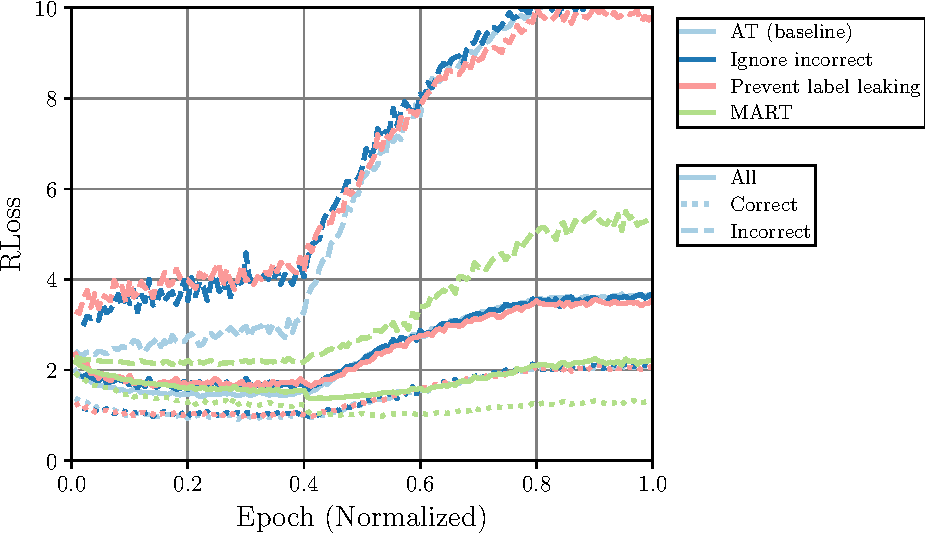
\includegraphics[width=0.425\textwidth]{plots_supp_understanding_incorrect2}
	\vspace*{-6px}
	\caption{\textbf{Approaches of Handling Incorrect Examples:} We plot test \RCE on all (solid), correctly classified (dotted) and incorrectly classified (dashed) examples throughout training. We consider our AT baseline ({\color{plot0}light blue}), ignoring incorrectly classified training examples in the \RCE computation during training ({\color{plot1}dark blue}) and preventing label leaking by computing adversarial examples against the \emph{predicted} labels during training ({\color{plot2}rose}). However, these ``simple'' approaches of tackling the high \RCE on incorrectly classified test examples are not successful in reducing robust overfitting. As outlined in the main paper, MART \cite{WangICLR2020} ({\color{plot3}green}) is able to dampen overfitting through an additional robust KL-loss weighted by confidence, see text.}
	\label{fig:supp-ii-pll}
	\vspace*{-6px}
\end{figure}
\begin{figure*}[t]
	\centering
	\begin{minipage}[t]{0.23\textwidth}
		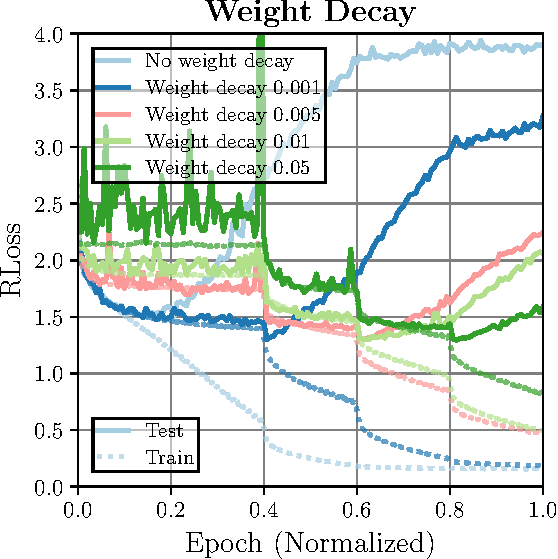
\includegraphics[width=\textwidth]{plots_supp_understanding_ablation_wd}
	\end{minipage}
	\begin{minipage}[t]{0.23\textwidth}
		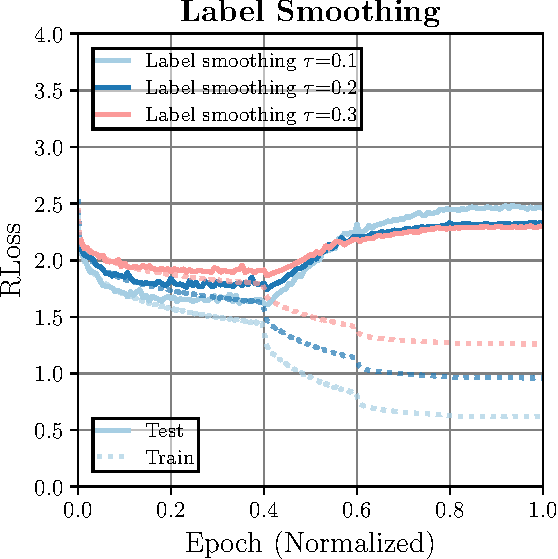
\includegraphics[width=\textwidth]{plots_supp_understanding_ablation_ls}
	\end{minipage}
	\begin{minipage}[t]{0.23\textwidth}
		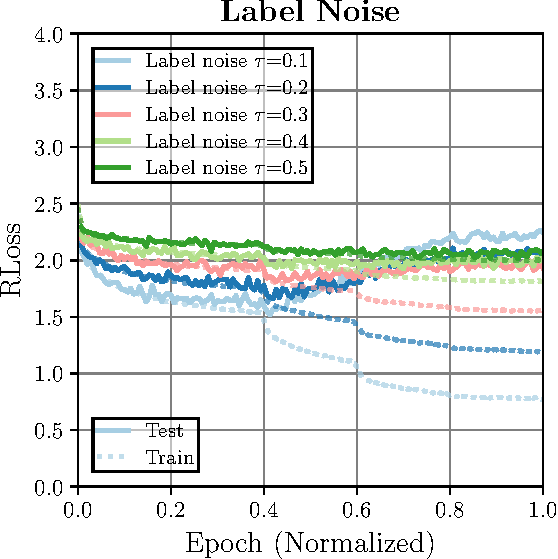
\includegraphics[width=\textwidth]{plots_main_understanding_ablation_ln}
	\end{minipage}
	\begin{minipage}[t]{0.23\textwidth}
		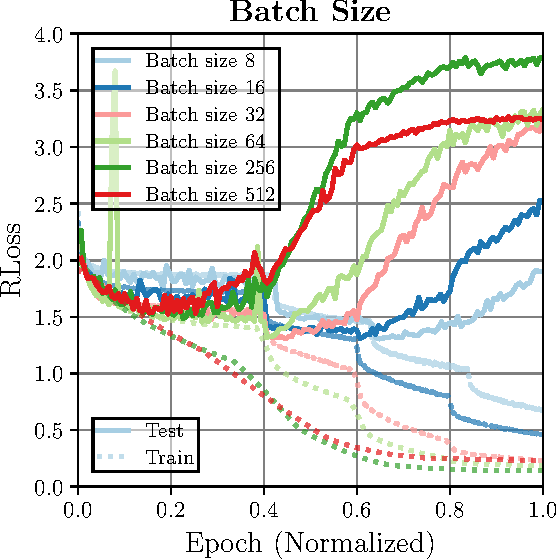
\includegraphics[width=\textwidth]{plots_supp_understanding_ablation_bs}
	\end{minipage}
	\\[2.5px]
	\begin{minipage}[t]{0.23\textwidth}
		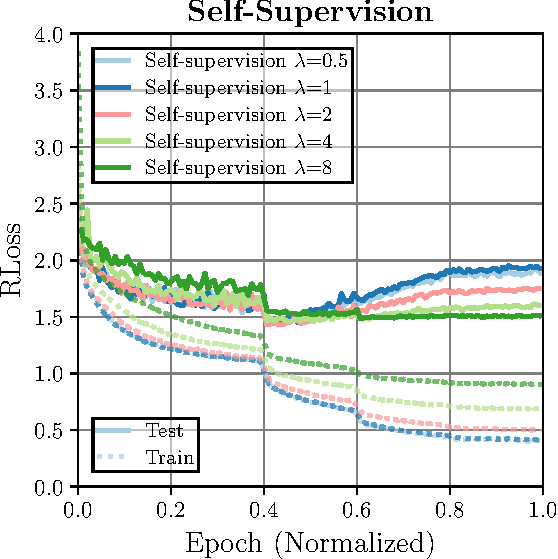
\includegraphics[width=\textwidth]{plots_supp_understanding_ablation_ssl}
	\end{minipage}
	\begin{minipage}[t]{0.23\textwidth}
		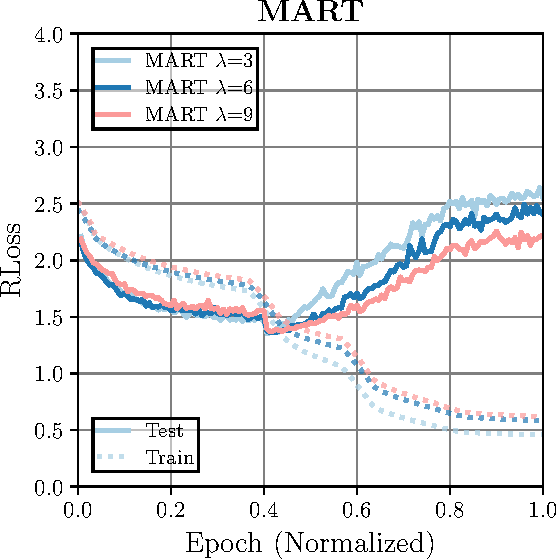
\includegraphics[width=\textwidth]{plots_supp_understanding_ablation_mart}
	\end{minipage}
	\begin{minipage}[t]{0.23\textwidth}
		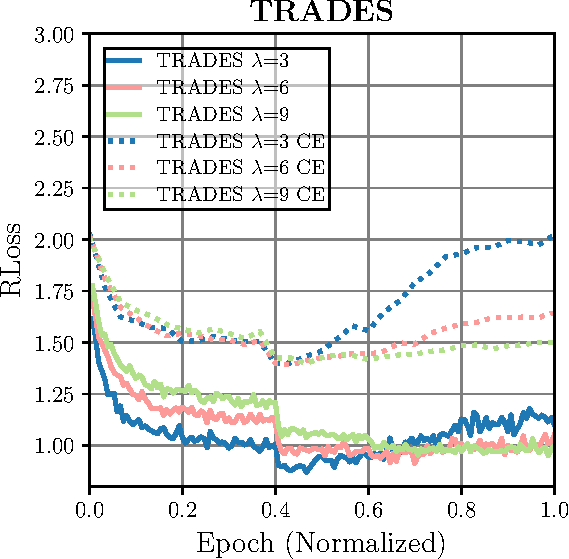
\includegraphics[width=\textwidth]{plots_supp_understanding_ablation_trades}
	\end{minipage}
	\begin{minipage}[t]{0.23\textwidth}
		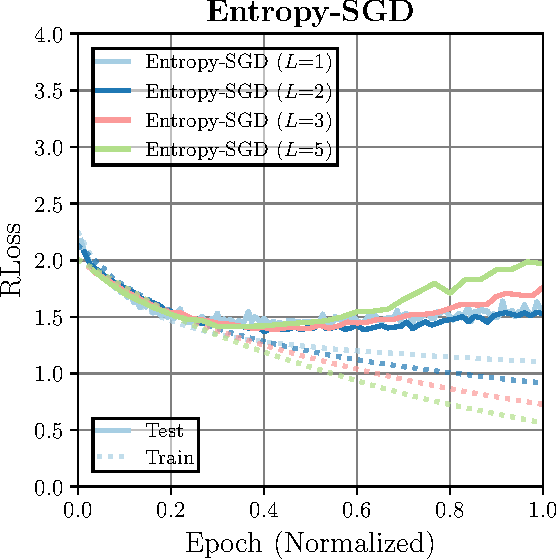
\includegraphics[width=\textwidth]{plots_supp_understanding_ablation_esgd}
	\end{minipage}
	\caption{\textbf{Training Curves for Varying Hyper-Parameters:} We plot \RCE for selected methods and hyper-parameters to demonstrate the impact of hyper-parameters on avoiding or reducing robust overfitting. Note that, for TRADES, we show both \RCE on adversarial examples computed by maximizing the KL-divergence in \eqnref{eq:supp-methods-trades} (solid) and on adversarial examples obtained by maximizing cross-entropy loss (``CE'', dotted).}
	\label{fig:supp-training-ablation}
\end{figure*}

\textbf{Activation functions:}
%
We consider three recently proposed activation functions: SiLU \cite{ElfwingNN2018}, MiSH \cite{MisraBMVC2020} and GeLU \cite{HendrycksARXIV2016}. These are defined as:
\begin{align}
	(\text{SiLU})\quad &x \sigma(x)\text{ with } \sigma(x) = \nicefrac{1}{(1 + \exp(-x))},\\
	(\text{MiSH})\quad &x \tanh(\log(1 + \exp(x))),\\
	(\text{GeLU})\quad &x \sigma(1.702 x).
\end{align}
All of these activation functions can be seen as smooth versions of the ReLU activation.
In \cite{SinglaARXIV2021}, some of these activation functions are argued to avoid robust overfitting due to lower curvature compared to ReLU.

\textbf{AT-AWP:}
%
AT with adversarial weight perturbations (AT-AWP) \cite{WuNIPS2020} computes adversarial weight perturbations \emph{on top} of adversarial examples to further regularize training. This is similar to our worst-case flatness measure of \RCE, however, adversarial examples and adversarial weights are computed sequentially, not jointly, and only one iteration is used to compute adversarial weights. Specifically, after computing adversarial examples $\tilde{x} = x + \delta$,
an adversarial weight perturbation $\nu$ is computed by solving
\begin{align}
	\max_{\nu \in B_\xi(w)} \mathcal{L}(f(\tilde{x}; w + \nu), y)
\end{align}
with $B_\xi(w)$ as in \eqnref{eq:supp-ball} using one iteration of gradient ascent with fixed step size of $\xi$. The gradient is normalized per layer as in \eqnref{eq:supp-normalization}.
We considered $\xi \in \{0.0005, 0.001, 0.005, 0.01, 0.015, 0.02\}$ and between $1$ and $7$ iterations and found that $\xi = 0.01$ and $1$ iteration works best (similar to \cite{WuNIPS2020}).

\textbf{TRADES:} \cite{ZhangICML2019} proposes an alternative formulation of AT that allows a better trade-off between adversarial robustness and (clean) accuracy. The loss to be minimized is
\begin{align}
	\begin{split}
		\mathcal{L}&(f(x;w), y)\\
		&+ \lambda \max_{\|\delta\|_\infty \leq \epsilon} \text{KL}(f(x;w), f(x + \delta;w)).\label{eq:supp-methods-trades}
	\end{split}
\end{align}
During training, adversarial examples are computed by maximizing the KL-divergence (instead of cross-entropy loss), \ie, using the second term in \eqnref{eq:supp-methods-trades}. Commonly $\lambda = 6$ is chosen, however, we additionally tried $\lambda \in \{1, 3, 6, 9\}$. We follow the official implementation\footnote{\url{https://github.com/yaodongyu/TRADES}}.

\begin{figure*}
	\centering
	\vspace*{-0.2cm}
	\begin{minipage}[t]{0.11\textwidth}
		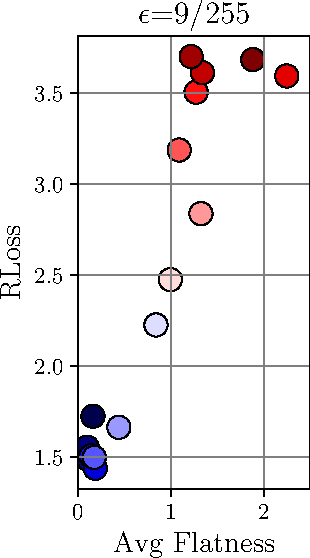
\includegraphics[height=3.25cm]{plots_supp_flatness_epochs_correlation_joint_eps}
	\end{minipage}
	\begin{minipage}[t]{0.12\textwidth}
		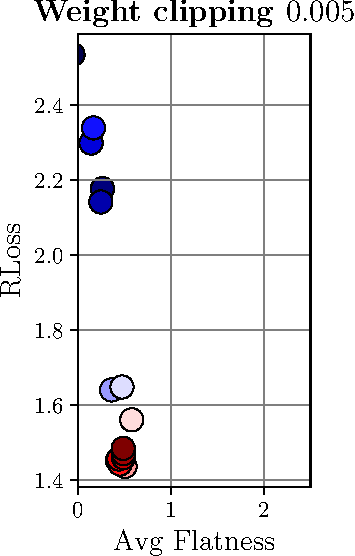
\includegraphics[height=3.25cm]{plots_supp_flatness_epochs_correlation_joint_0005p}
	\end{minipage}
	\begin{minipage}[t]{0.11\textwidth}
		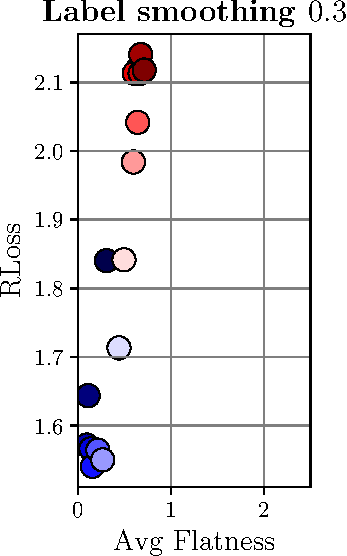
\includegraphics[height=3.25cm]{plots_supp_flatness_epochs_correlation_joint_ls03}
	\end{minipage}
	\begin{minipage}[t]{0.11\textwidth}
		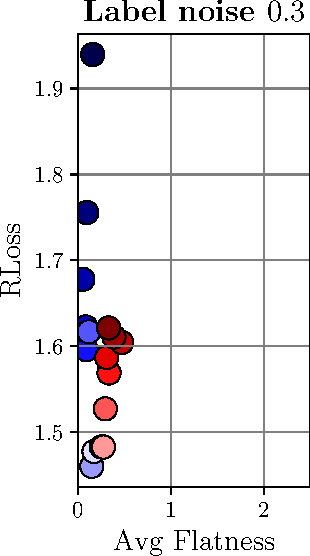
\includegraphics[height=3.25cm]{plots_supp_flatness_epochs_correlation_joint_ln03}
	\end{minipage}
	\begin{minipage}[t]{0.11\textwidth}
		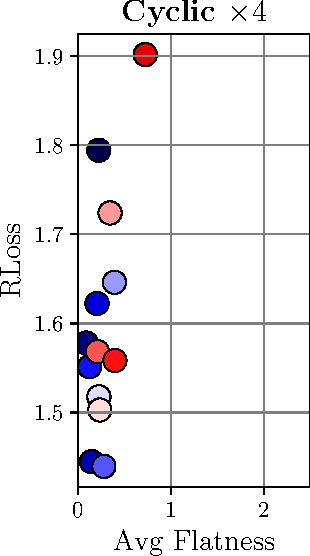
\includegraphics[height=3.25cm]{plots_supp_flatness_epochs_correlation_joint_cyc4}
	\end{minipage}
	\begin{minipage}[t]{0.11\textwidth}
		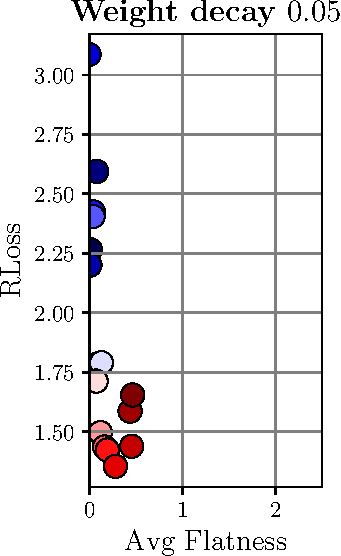
\includegraphics[height=3.25cm]{plots_supp_flatness_epochs_correlation_joint_wd005}
	\end{minipage}
	\begin{minipage}[t]{0.145\textwidth}
		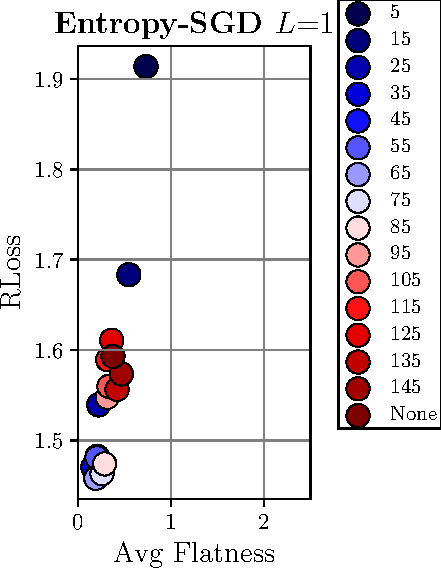
\includegraphics[height=3.25cm]{plots_supp_flatness_epochs_correlation_joint_esgd1}
	\end{minipage}
	\\[2.5px]
	
	\begin{minipage}[t]{0.12\textwidth} 
		\hphantom{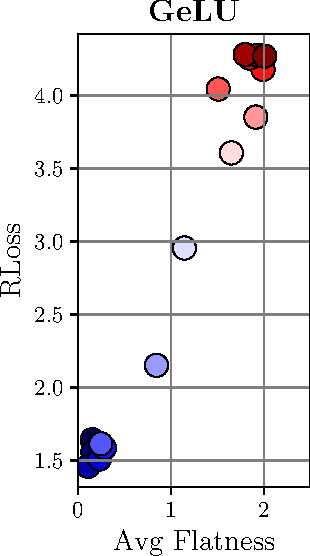
\includegraphics[height=3.25cm]{plots_supp_flatness_epochs_correlation_joint_gelu}}
	\end{minipage}
	\begin{minipage}[t]{0.11\textwidth}
		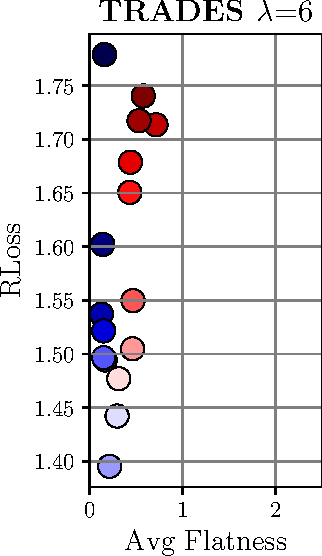
\includegraphics[height=3.25cm]{plots_supp_flatness_epochs_correlation_joint_trades6}
	\end{minipage}
	\begin{minipage}[t]{0.11\textwidth}
		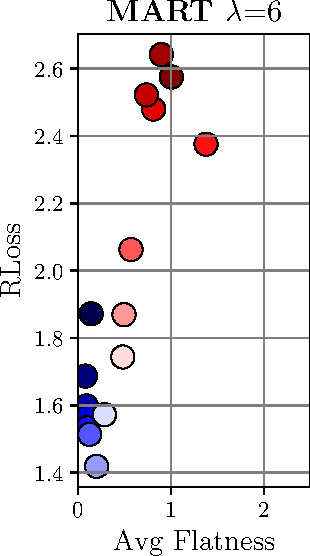
\includegraphics[height=3.25cm]{plots_supp_flatness_epochs_correlation_joint_mart6}
	\end{minipage}
	\begin{minipage}[t]{0.11\textwidth}
		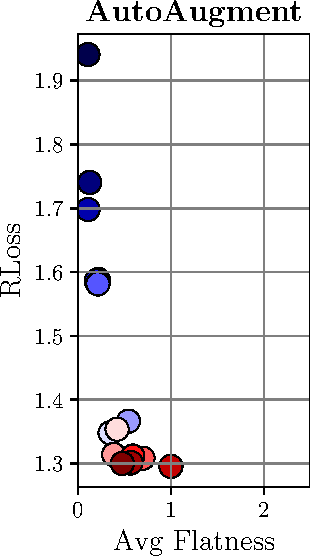
\includegraphics[height=3.25cm]{plots_supp_flatness_epochs_correlation_joint_aa}
	\end{minipage}
	\begin{minipage}[t]{0.11\textwidth}
		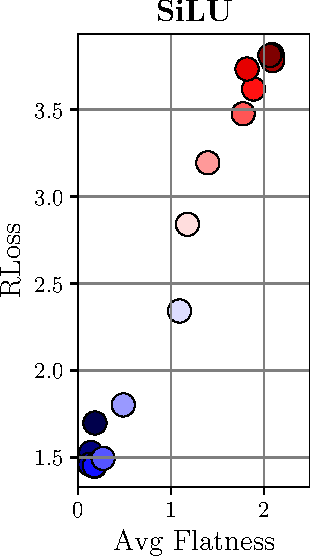
\includegraphics[height=3.25cm]{plots_supp_flatness_epochs_correlation_joint_silu}
	\end{minipage}
	\begin{minipage}[t]{0.11\textwidth}
		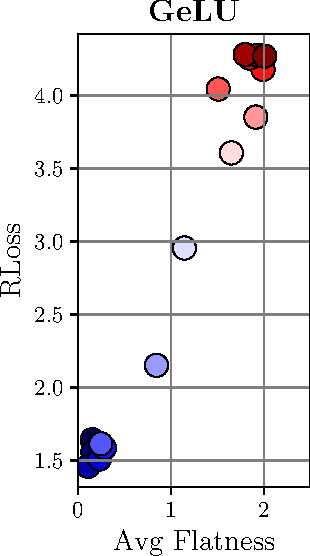
\includegraphics[height=3.25cm]{plots_supp_flatness_epochs_correlation_joint_gelu}
	\end{minipage}
	\begin{minipage}[t]{0.14\textwidth}
		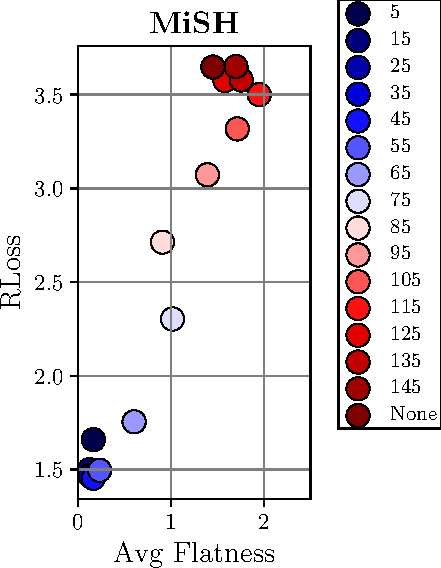
\includegraphics[height=3.25cm]{plots_supp_flatness_epochs_correlation_joint_mish}
	\end{minipage}
	\vspace*{-6px}
	\caption{\textbf{Flatness Throughout Training:} Complementary to the main paper, we plot \RCE against average-case flatness in \RCE for selected methods throughout training epochs. \red{Early epochs are shown in {\color{blue!60!black}dark blue}, late epochs are shown in {\color{red!60!black}dark red}.} For cyclic learning rate, we show $4$ cycles with a total of $120$ epochs. For many methods not avoiding robust overfitting, flatness decreases alongside an increase in \RCE during overfitting. Using, \eg, AutoAugment, label noise or Entropy-SGD, in contrast, both effects are reduced.}
	\label{fig:supp-methods-flatness-epochs}
	\vspace*{-6px}
\end{figure*}

\textbf{MART} \cite{WangICLR2020} explicitly addresses the problem of incorrectly classified examples during training. First, the cross-entropy loss $\mathcal{L}$ for training is replaced using a binary cross-entropy loss $\mathcal{L}_{\text{bin}}$, \ie, classifying correct class vs\onedot most-confident ``other'' class:
\begin{align}
	\begin{split}
		\mathcal{L}_{\text{bin}}(f(x; w), y) =& -\log(f_y(x;w))\\
		& - \log(1 - \max_{y' \neq y} f_{y'}(x; w)).
	\end{split}
\end{align}
Second, the KL-divergence used in TRADES in \eqnref{eq:supp-methods-trades} is combined with a confidence-based weight:
\begin{align}
	\begin{split}
		\mathcal{L}_{\text{bin}}&(f(\tilde{x}; w), y)\\ &+ \lambda \text{KL}(f(x;w), f(\tilde{x}; w)() (1 - f_y(x; w))
	\end{split}
\end{align}
Adversarial examples are still computed by maximizing regular cross-entropy loss. We follow the official implementation\footnote{\url{https://github.com/YisenWang/MART}}. MART is successful in reducing robust overfitting on incorrectly classified examples, as shown in \figref{fig:supp-ii-pll}.

\textbf{PGD-$\tau$:}
%
In \cite{ZhangARXIV2020}, a variant of PGD is proposed for AT: PGD-$\tau$ stops maximization $\tau$ iterations \emph{after} the label flipped. This is supposed to find ``friendlier'' adversarial examples that can be used for AT. Note that $\tau = 0$ also does \emph{not} compute adversarial examples on incorrectly classified training examples. We consider $\tau \in \{0, 1, 2, 3\}$.

\textbf{Self-Supervision:} Following \cite{HendrycksNIPS2019}, we implement AT using rotation-prediction as \emph{additional} self-supervised task. Note, however, that no additional (unlabeled) training examples are used. Specifically, the following learning problem is tackled:
\begin{align}
	\begin{split}
		\max&_{\|\delta\|_\infty \leq \epsilon} \mathcal{L}(f(x + \delta;w), y)\\
		&+ \lambda \max_{\|\delta\|_\infty \leq \epsilon} \mathcal{L}(f(\text{rot}(x + \delta, r); w), y_{r})\\
		&r\in\{0, 90, 180, 270\}, y_r \in \{0, 1, 2, 3\}
	\end{split}
\end{align}
where $\text{rot}(x, r)$ rotates the training example $x$ by $r$ degrees.
In practice, we split every batch in half: The first half uses the original training examples with correct labels. Examples in the second half are rotated randomly by $\{0, 90, 180, 270\}$ degrees, and the labels correspond to the rotation (\ie, $\{0, 1, 2, 3\}$). Adversarial examples are computed against the true or rotation-based labels. Note that, in contrast to common practice \cite{SohnARXIV2020}, we do \emph{not} predict all four possible rotations every batch, but just one randomly drawn per example. We still use $150$ epochs in total. We consider $\lambda \in \{0.5, 1, 2, 4, 8\}$.
 
\textbf{Additional Unlabeled Examples:} As proposed in \cite{CarmonNIPS2019,UesatoNIPS2019}, we also consider additional, pseudo-labeled examples during training. We use the provided pseudo-labeled data from \cite{CarmonNIPS2019} and split each batch in half: using $50\%$ original \CifarT training examples, and $50\%$ pseudo-labeled training examples from \cite{CarmonNIPS2019}. We still use $150$ epochs in total. We follow the official PyTorch implementation\footnote{\url{https://github.com/yaircarmon/semisup-adv}}.

\subsection{Training Curves}
\label{sec:supp-methods-ablation}

\figref{fig:supp-training-ablation} shows (test) \RCE throughout training for selected methods and hyper-parameters. Across all methods, we found that hyper-parameters have a large impact on robust overfitting. For example, weight decay or smaller batch sizes can reduce and delay robust overfitting considerably if regularization is ``strong'' enough, \ie, large weight decay or low batch size (to induce more randomness). For the other methods, difference between hyper-parameters is more subtle. However, across all cases, reduced overfitting generally goes hand in hand with higher \RCE on training examples, \ie, the robust generalization gap is reduced. This indicates that avoiding convergence on training examples plays an important role in avoiding robust overfitting.

Training curves for all methods are shown in \figref{fig:supp-training-curves}.

\subsection{Flatness for Methods}
\label{sec:supp-methods-flatness}

\begin{figure*}[t]
\begin{minipage}{\textwidth}
	\centering
	\vspace*{-0.2cm}
	\hspace*{-0.4cm}
	\begin{minipage}[t]{0.18\textwidth}
		\vspace*{0px}
		
		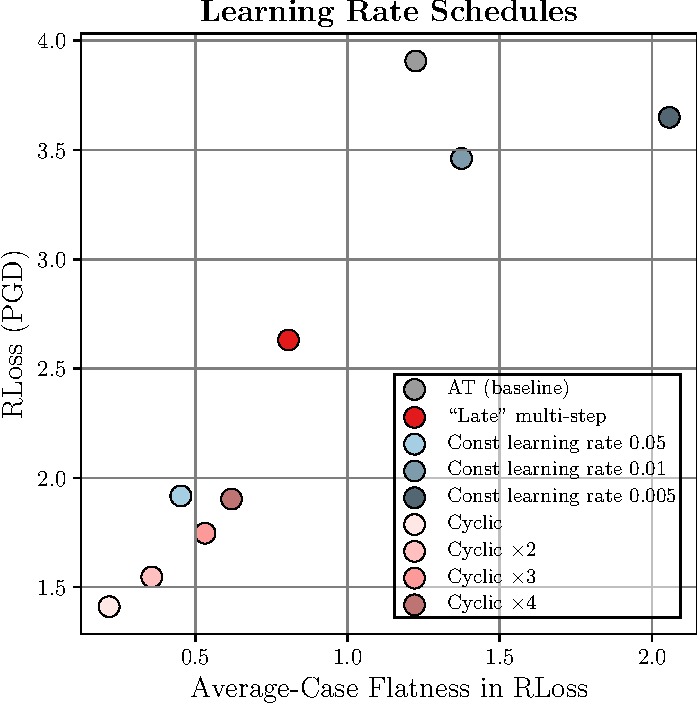
\includegraphics[width=\textwidth]{plots_supp_flatness_correlation_seq_loss_methods_lr}
	\end{minipage}
	\begin{minipage}[t]{0.18\textwidth}
		\vspace*{0px}
				
		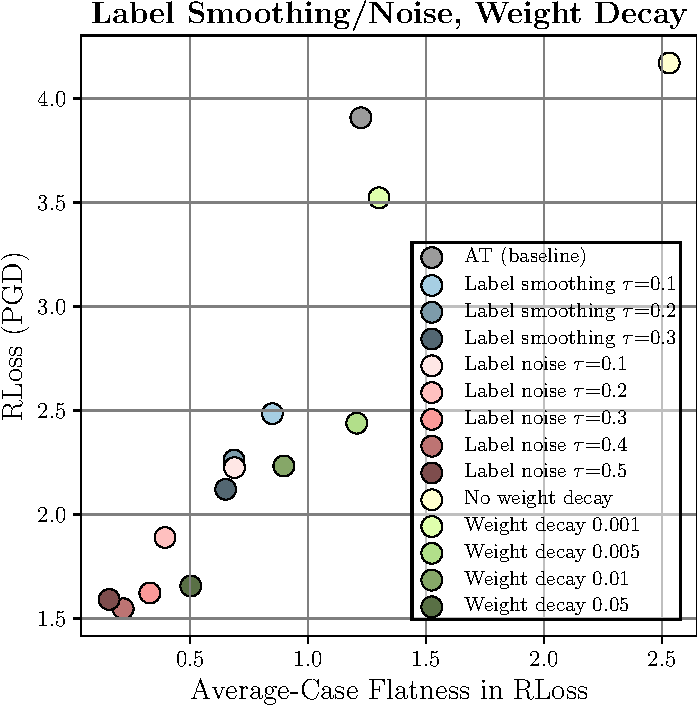
\includegraphics[width=\textwidth]{plots_supp_flatness_correlation_seq_loss_methods_ls}
	\end{minipage}
	\begin{minipage}[t]{0.18\textwidth}
		\vspace*{0px}
				
		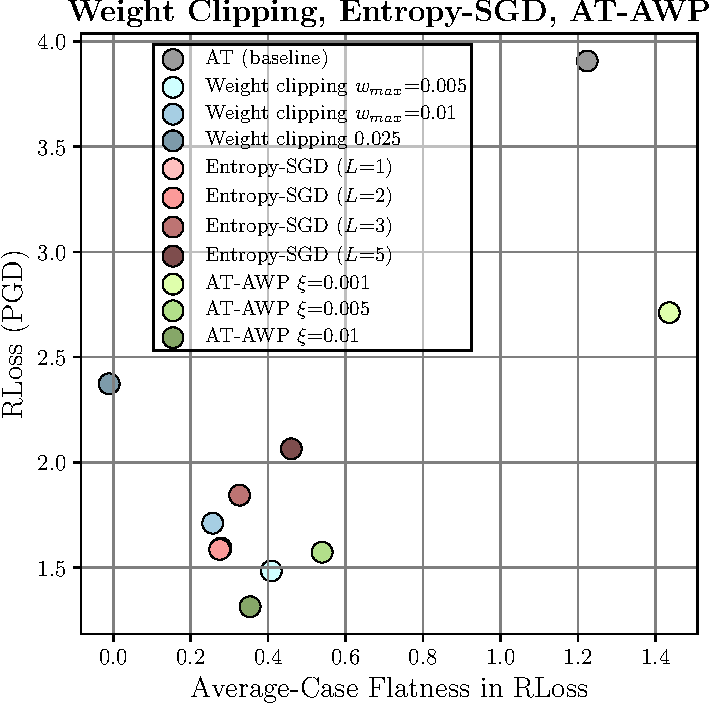
\includegraphics[width=\textwidth]{plots_supp_flatness_correlation_seq_loss_methods_flat}
	\end{minipage}
	\begin{minipage}[t]{0.26\textwidth}
		\vspace*{0px}
				
		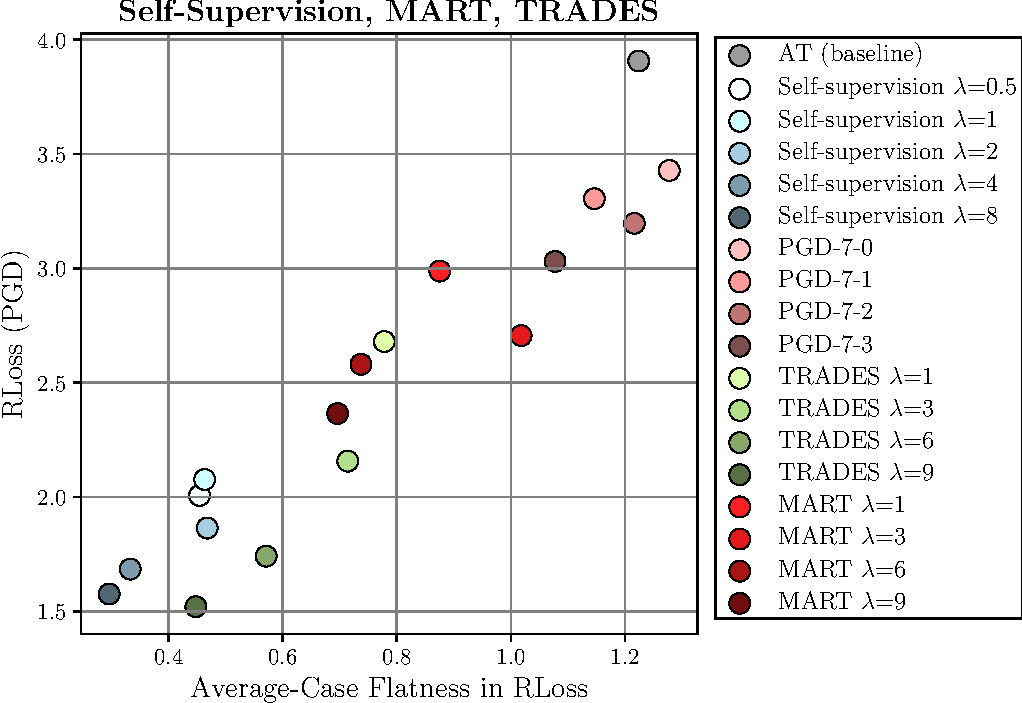
\includegraphics[width=1\textwidth]{plots_supp_flatness_correlation_seq_loss_methods_at}
	\end{minipage}
	\begin{minipage}[t]{0.01\textwidth}
		\vspace*{0px}
		
		\hspace*{4px}{\color{black!75}\rule{0.65px}{3.15cm}}
	\end{minipage}
	\begin{minipage}[t]{0.18\textwidth}
		\vspace*{0px}
				 
		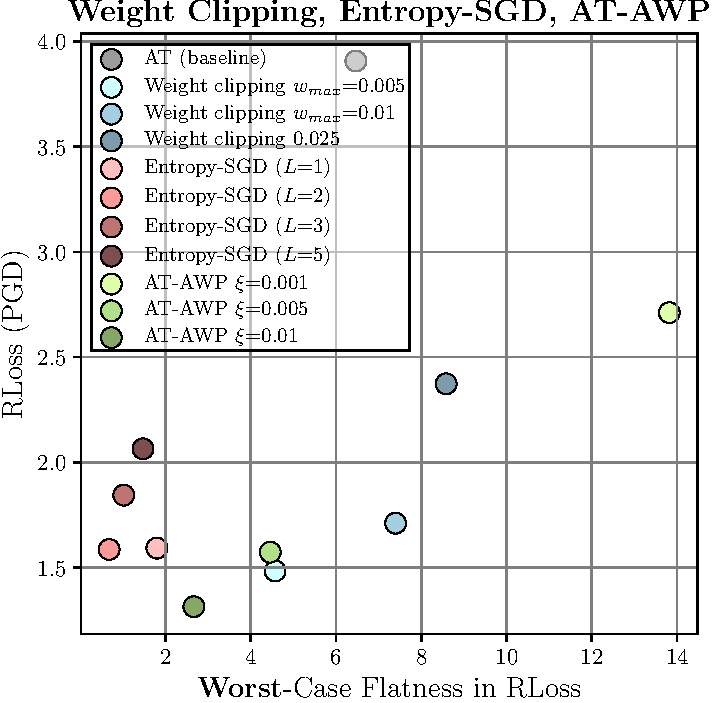
\includegraphics[width=1\textwidth]{plots_supp_flatness_correlation_joint_loss_methods_flat}
	\end{minipage}

	\vspace*{-6px}
	\captionof{figure}{\textbf{Robustness and Flatness for Varying Hyper-Parameters:} \textbf{Left:} \RCE (y-axis) plotted against average-case flatness of \RCE (x-axis) for various groups of methods: learning rate schedules (left), label smoothing/noise and weight decay (middle left), weight clipping, Entropy-SGD and AT-AWP (middle right) as well as AT with self-supervision, MART and TRADES (right). As outlined in \secref{sec:supp-methods}, we considered multiple hyper-parameter settings per method and show that favorable hyper-parameters in terms of adversarial robustness also result in improved flatness. That is, in most cases, varying hyper-parameters creates (roughly) a diagonal line in these plots. Interestingly, weight clipping can be considered an outlier: adversarial robustness improves while \emph{average-case} flatness \emph{reduces}. \textbf{Right:} \RCE (y-axis) plotted against \emph{worst-case} flatness in \RCE (x-axis). Here, flatness for weight clipping aligns well with \RCE.}
	\label{fig:supp-flatness-methods}
	\vspace*{12px}
\end{minipage}
\end{figure*}


\textbf{Flatness Throughout Training:}
%
\figref{fig:supp-methods-flatness-epochs} shows \RCE (y-axis) plotted against average-case flatness in \RCE (x-axis) throughout training, \ie, over epochs ({\color{blue!50!black}dark blue} to {\color{red!50!black}dark red}), for methods not shown in the main paper. Strikingly, using higher $\epsilon{=}\nicefrac{9}{255}$ or alternative activation functions (SiLU \cite{ElfwingNN2018}, GeLU \cite{HendrycksARXIV2016} or MiSH \cite{MisraBMVC2020}) affect neither robust overfitting nor flatness significantly. Interestingly, as discussed in the main paper, label smoothing avoids sharper minima during overfitting, but does \emph{not} avoid an increased \RCE. Methods that consistently reduce or avoid robust overfitting, \eg, weight clipping, label noise, strong weight decay or AutoAugment, avoid both the increase in \RCE as well as worse flatness. Clearly, the observations from the main paper are confirmed: flatness usually reduces alongside \RCE in robust overfitting.

\textbf{Flatness Across Hyper-Parameters:}
%
In \figref{fig:supp-flatness-methods}, we consider flatness when changing hyper-parameters of selected methods. As before, we plot \RCE (y-axis) against average-case flatness in \RCE (x-axis) for various groups of methods: learning rate schedules (first column), label smoothing/noise and weight decay (second column), methods explicitly improving flatness, \ie, weight clipping, Entropy-SGD and AT-AWP (third column), as well as self-supervision, MART and TRADES (fourth column). Except for weight clipping, hyper-parameter settings with improved adversarial robustness also favor flatter minima. In most cases, this relationship follows a clear, diagonal line. For weight clipping, in contrast, the relationship is reversed: improved flatness reduces \RCE. Thus, \figref{fig:supp-flatness-methods} (fifth column) considers worst-case flatness in \RCE. Here, ``stronger'' weight clipping improves both robustness \emph{and} flatness. This supports our discussion in the main paper: methods need at least ``some kind'' of flatness, average- or worst-case, in order to improve adversarial robustness.

\section{Results in Tabular Form}
\label{sec:supp-results}

\tabref{tab:supp-table-error} and \ref{tab:supp-table-loss} report the quantitative results from all our experiments. Besides flatness in \RCE, we also report both average- and worst-case flatness in (clean) \CE. As described in the main paper, we use $\xi = 0.5$ for average-case flatness and $\xi = 0.003$ for worst-case flatness. In \tabref{tab:supp-table-error}, methods are sorted (in ascending order) by \RTE against AutoAttack \cite{CroceICML2020}. Additionally, we split all methods into four groups: \colorbox{colorbrewer3!15}{good}, \colorbox{colorbrewer5!15}{average}, \colorbox{colorbrewer1!15}{poor} and \colorbox{colorbrewer0!15}{worse} robustness at $57\%$, $60\%$ and $62.8\%$ \RTE. These thresholds correspond roughly to the $30\%$ and $70\%$ percentile of all methods with $\RTE \leq 62.8\%$. As our AT baseline obtains $62.8\%$ \RTE, we group all methods with higher \RTE than $62.8\%$ in \colorbox{colorbrewer0!15}{worse} robustness. In \tabref{tab:supp-table-loss}, methods are sorted (in ascending order) by \RCE against PGD. Finally, \tabref{tab:supp-table-robustbench-error} and \ref{tab:supp-table-robustbench-loss} report \RTE and \RCE, together with our average- and worst-case flatness (of \RCE) measures for the evaluated, pre-trained models from RobustBench \cite{CroceARXIV2020b}.

\newpage
\clearpage
\begin{figure*}
\begin{minipage}{\textwidth}
	\centering
	\scriptsize
	{
	\begin{tabularx}{\textwidth}{|X|c|c|c||c|c|c||c|c|}
		\hline
		Model & \multicolumn{3}{c||}{\bfseries Test Robustness} & \multicolumn{3}{c||}{\bfseries Train Robustness} & \multicolumn{2}{c|}{\bfseries Flatness}\\
		\hline
		(sorted by \RCE on AA) & \TE & \RTE & \RTE & \TE & \RTE & \RTE & Avg & Worst\\
		(PGD = PGD-$20$, $10$ restarts) & (test) & (test) & (test) & (train) & (train) & (train) & \RCE & \RCE\\
		(AA = AutoAttack \cite{CroceARXIV2020}) && (PGD) & (AA) && (PGD) & (AA) &&\\
		\hline
		\hline
		Carmon et al. [16] & 10.31 & 37.6 & 40.8 & 1.93 & 16.8 & 19.2 & 0.7 & 0.34\\
		Engstrom et al. [36] & 12.97 & 45.3 & 49.2 & 6.71 & 33.1 & 36.3 & 0.23 & 0.51\\
		Pang et al. [93] & 14.87 & 36.6 & 45.8 & 7.79 & 20.5 & 28.6 & 0.08 & 0.07\\
		Wang [238] & 12.5 & 37.1 & 42.8 & 8.07 & 24.8 & 32.1 & 0.61 & 0.34\\
		Wong et al. [131] & 16.66 & 54.4 & 57.6 & 11.86 & 44.9 & 49.2 & 0.3 & 0.16\\
		Wu et al. [133] & 14.64 & 41.5 & 43.9 & 2.2 & 14.5 & 16.5 & 0.49 & 0.09\\
		Zhang et al. [148] & 15.08 & 44.1 & 46.4 & 7.83 & 29.9 & 33.6 & 0.61 & 0.43\\
		Zhang et al. [149] & 15.48 & 43 & 47.2 & 4.85 & 26.3 & 30.1 & 0.51 & 0.13\\
		\hline
	\end{tabularx} 
	}
	\vspace*{-8px}
	\captionof{table}{\textbf{RobustBench \cite{CroceARXIV2020b}: \TE, \RTE and Flatness in \RCE:} \TE and \RTE on train and test examples as well as average- and worst-case flatness in \RCE for pre-trained models from RobustBench. In contrast to \tabref{tab:supp-table-error}, the RobustBench models were obtained using early stopping.}
	\label{tab:supp-table-robustbench-error}
	\vspace*{12px}
\end{minipage}
\begin{minipage}{\textwidth}
	\centering
	\scriptsize
	{
	\begin{tabularx}{\textwidth}{|X|c|c|c||c|c|c||c|c|}
		\hline
		Model & \multicolumn{3}{c||}{\bfseries Test Robustness} & \multicolumn{3}{c||}{\bfseries Train Robustness} & \multicolumn{2}{c|}{\bfseries Flatness}\\
		\hline
		(sorted by \RCE on AA) & \CE & \RCE & \RCE & \CE & \RCE & \RCE & Avg & Worst\\
		(PGD = PGD-$20$, $10$ restarts) & (test) & (test) & (test) & (train) & (train) & (train) & \RCE & \RCE\\
		(AA = AutoAttack \cite{CroceARXIV2020}) && (PGD) & (AA) && (PGD) & (AA) &&\\
		\hline
		\hline
		Carmon et al. [16] & 0.53 & 1.02 & 0.63 & 0.36 & 0.62 & 0.41 & 0.7 & 0.34\\
		Engstrom et al. [36] & 0.44 & 1.25 & 0.59 & 0.29 & 0.82 & 0.41 & 0.23 & 0.51\\
		Pang et al. [93] & 1.84 & 1.98 & 1.86 & 1.8 & 1.91 & 1.8 & 0.08 & 0.07\\
		Wang [128] & 0.64 & 1.11 & 0.73 & 0.54 & 0.9 & 0.6 & 0.61 & 0.34\\
		Wong et al. [131] & 0.57 & 1.37 & 0.73 & 0.46 & 1.11 & 0.61 & 0.3 & 0.16\\
		Wu et al. [133] & 0.63 & 1.13 & 0.72 & 0.37 & 0.61 & 0.41 & 0.49 & 0.09\\
		Zhang et al. [148] & 0.55 & 1.19 & 0.66 & 0.39 & 0.83 & 0.48 & 0.61 & 0.43\\
		Zhang et al. [149] & 0.85 & 1.27 & 0.93 & 0.71 & 1.01 & 0.76 & 0.51 & 0.13\\
		\hline
	\end{tabularx} 
	}
	\vspace*{-8px}
	\captionof{table}{\textbf{RobustBench \cite{CroceARXIV2020b}: \emph{\CE, \RCE} and Flatness in \RCE:} \CE and \RCE on train and test examples as well as average- and worst-case flatness in \RCE for pre-trained models from RobustBench. In contrast to \tabref{tab:supp-table-loss}, the RobustBench models were obtained using early stopping.}
	\label{tab:supp-table-robustbench-loss}
	\vspace*{-6px}
\end{minipage}
\end{figure*}
\FloatBarrier
\begin{figure*}[t]
	\centering
	\begin{minipage}[t]{0.19\textwidth}
		\vspace*{0px}
		
		\includegraphics[height=1.8cm]{plots_supp_training_curves_eps_loss}
		
		\hspace*{-0.25cm}
		\includegraphics[height=1.8cm]{plots_supp_training_curves_eps_error}
	\end{minipage}
	\begin{minipage}[t]{0.19\textwidth}
		\vspace*{0px}
		
		\includegraphics[height=1.8cm]{plots_supp_training_curves_i5_loss}
		
		\hspace*{-0.25cm}
		\includegraphics[height=1.8cm]{plots_supp_training_curves_i5_error}
	\end{minipage}
	\begin{minipage}[t]{0.19\textwidth}
		\vspace*{0px}
		
		\includegraphics[height=1.8cm]{plots_supp_training_curves_i14_loss}
		
		\hspace*{-0.25cm}
		\includegraphics[height=1.8cm]{plots_supp_training_curves_i14_error}
	\end{minipage}
	\begin{minipage}[t]{0.19\textwidth}
		\vspace*{0px}
		
		\includegraphics[height=1.8cm]{plots_supp_training_curves_ii_loss}
		
		\hspace*{-0.25cm}
		\includegraphics[height=1.8cm]{plots_supp_training_curves_ii_error}
	\end{minipage}
	\begin{minipage}[t]{0.19\textwidth}
		\vspace*{0px}
		
		\includegraphics[height=1.8cm]{plots_supp_training_curves_pll_loss}
		
		\hspace*{-0.25cm}
		\includegraphics[height=1.8cm]{plots_supp_training_curves_pll_error}
	\end{minipage}
	\\[2.5px]
	
	\begin{minipage}[t]{0.19\textwidth}
		\vspace*{0px}
		
		\includegraphics[height=1.8cm]{plots_supp_training_curves_0005p_loss}
		
		\hspace*{-0.25cm}
		\includegraphics[height=1.8cm]{plots_supp_training_curves_0005p_error}
	\end{minipage}
	\begin{minipage}[t]{0.19\textwidth}
		\vspace*{0px}
		
		\includegraphics[height=1.8cm]{plots_supp_training_curves_ls03_loss}
		
		\hspace*{-0.25cm}
		\includegraphics[height=1.8cm]{plots_supp_training_curves_ls03_error}
	\end{minipage}
	\begin{minipage}[t]{0.19\textwidth}
		\vspace*{0px}
		
		\includegraphics[height=1.8cm]{plots_supp_training_curves_ln03_loss}
		
		\hspace*{-0.25cm}
		\includegraphics[height=1.8cm]{plots_supp_training_curves_ln03_error}
	\end{minipage}
	\begin{minipage}[t]{0.19\textwidth}
		\vspace*{0px}
		
		\includegraphics[height=1.8cm]{plots_supp_training_curves_late_loss}
		
		\hspace*{-0.25cm}
		\includegraphics[height=1.8cm]{plots_supp_training_curves_late_error}
	\end{minipage}
	\begin{minipage}[t]{0.19\textwidth}
		\vspace*{0px}
		
		\includegraphics[height=1.8cm]{plots_supp_training_curves_const_loss}
		
		\hspace*{-0.25cm}
		\includegraphics[height=1.8cm]{plots_supp_training_curves_const_error}
	\end{minipage}
	\\[2.5px]
		
	\begin{minipage}[t]{0.19\textwidth}
		\vspace*{0px}
		
		\includegraphics[height=1.8cm]{plots_supp_training_curves_cyc4_loss}
		
		\hspace*{-0.25cm}
		\includegraphics[height=1.8cm]{plots_supp_training_curves_cyc4_error}
	\end{minipage}
	\begin{minipage}[t]{0.19\textwidth}
		\vspace*{0px}
		 
		\includegraphics[height=1.8cm]{plots_supp_training_curves_lr02_loss}
		
		\hspace*{-0.25cm}
		\includegraphics[height=1.8cm]{plots_supp_training_curves_lr02_error}
	\end{minipage}
	\begin{minipage}[t]{0.19\textwidth}
		\vspace*{0px}
		
		\includegraphics[height=1.8cm]{plots_supp_training_curves_b16_loss}
		
		\hspace*{-0.25cm}
		\includegraphics[height=1.8cm]{plots_supp_training_curves_b16_error}
	\end{minipage}
	\begin{minipage}[t]{0.19\textwidth}
		\vspace*{0px}
		
		\includegraphics[height=1.8cm]{plots_supp_training_curves_b512_loss}
		
		\hspace*{-0.25cm}
		\includegraphics[height=1.8cm]{plots_supp_training_curves_b512_error}
	\end{minipage}
	\begin{minipage}[t]{0.19\textwidth}
		\vspace*{0px}
		
		\includegraphics[height=1.8cm]{plots_supp_training_curves_nowd_loss}
		
		\hspace*{-0.25cm}
		\includegraphics[height=1.8cm]{plots_supp_training_curves_nowd_error}
	\end{minipage}
	\\[2.5px]
	\begin{minipage}[t]{0.19\textwidth}
		\vspace*{0px}
		
		\includegraphics[height=1.8cm]{plots_supp_training_curves_wd005_loss}
		
		\hspace*{-0.25cm}
		\includegraphics[height=1.8cm]{plots_supp_training_curves_wd005_error}
	\end{minipage}
	\begin{minipage}[t]{0.19\textwidth}
		\vspace*{0px}
		
		\includegraphics[height=1.8cm]{plots_supp_training_curves_esgd1_loss}
		
		\hspace*{-0.25cm}
		\includegraphics[height=1.8cm]{plots_supp_training_curves_esgd1_error}
	\end{minipage}
	\begin{minipage}[t]{0.19\textwidth}
		\vspace*{0px}
		
		\includegraphics[height=1.8cm]{plots_supp_training_curves_tau0_loss}
		
		\hspace*{-0.15cm}
		\includegraphics[height=1.8cm]{plots_supp_training_curves_tau0_error}
	\end{minipage}
	\begin{minipage}[t]{0.19\textwidth}
		\vspace*{0px}
		
		\includegraphics[height=1.8cm]{plots_supp_training_curves_trades6_loss}
		
		\hspace*{-0.25cm}
		\includegraphics[height=1.8cm]{plots_supp_training_curves_trades6_error}
	\end{minipage}
	\begin{minipage}[t]{0.19\textwidth}
		\vspace*{0px}
		
		\includegraphics[height=1.8cm]{plots_supp_training_curves_mart6_loss}
		
		\hspace*{-0.25cm}
		\includegraphics[height=1.8cm]{plots_supp_training_curves_mart6_error}
	\end{minipage}
	\\[2.5px]
	
	\begin{minipage}[t]{0.19\textwidth}
		\vspace*{0px}
		
		\includegraphics[height=1.8cm]{plots_supp_training_curves_aa_loss}
		
		\hspace*{-0.15cm}
		\includegraphics[height=1.8cm]{plots_supp_training_curves_aa_error}
	\end{minipage}
	\begin{minipage}[t]{0.19\textwidth}
		\vspace*{0px}
		
		\includegraphics[height=1.8cm]{plots_supp_training_curves_500k_loss}
		
		\hspace*{-0.25cm}
		\includegraphics[height=1.8cm]{plots_supp_training_curves_500k_error}
	\end{minipage}
	\begin{minipage}[t]{0.19\textwidth}
		\vspace*{0px}
		
		\includegraphics[height=1.8cm]{plots_supp_training_curves_silu_loss}
		
		\hspace*{-0.25cm}
		\includegraphics[height=1.8cm]{plots_supp_training_curves_silu_error}
	\end{minipage}
	\begin{minipage}[t]{0.19\textwidth}
		\vspace*{0px}
		
		\includegraphics[height=1.8cm]{plots_supp_training_curves_gelu_loss}
		
		\hspace*{-0.25cm}
		\includegraphics[height=1.8cm]{plots_supp_training_curves_gelu_error}
	\end{minipage}
	\begin{minipage}[t]{0.19\textwidth}
		\vspace*{0px}
		
		\includegraphics[height=1.8cm]{plots_supp_training_curves_mish_loss}
		
		\hspace*{-0.25cm}
		\includegraphics[height=1.8cm]{plots_supp_training_curves_mish_error}
	\end{minipage}
	\\[2.5px]
	
	\begin{minipage}[t]{0.19\textwidth}
		\vspace*{0px}
		
		\includegraphics[height=1.8cm]{plots_supp_training_curves_dropout_loss}
		
		\hspace*{-0.15cm}
		\includegraphics[height=1.8cm]{plots_supp_training_curves_dropout_error}
	\end{minipage}
	\begin{minipage}[t]{0.19\textwidth}
		\vspace*{0px}
		
		\includegraphics[height=1.8cm]{plots_supp_training_curves_ssl4_loss}
		
		\hspace*{-0.25cm}
		\includegraphics[height=1.8cm]{plots_supp_training_curves_ssl4_error}
	\end{minipage}
	\begin{minipage}[t]{0.19\textwidth}
		\vspace*{0px}
		
		\includegraphics[height=1.8cm]{plots_supp_training_curves_awit001_loss}
		
		\hspace*{-0cm}
		\includegraphics[height=1.8cm]{plots_supp_training_curves_awit001_error}
	\end{minipage}
	\begin{minipage}[t]{0.01\textwidth}
		\vspace*{0px}
		
		\hfill
	\end{minipage}
	\begin{minipage}[t]{0.38\textwidth}
		\vspace*{4px}
		
		\caption{\textbf{Training Curves:} Test and train \RCE (top) and \RTE (bottom), including \RTE for early stopping, for all considered methods with selected hyper-parameters. \textbf{*} Train and test \RCE correspond to the attacks used during training, \eg, PGD-$\tau$ or maximizing KL-divergence for TRADES. \textbf{$\dagger$} Reported \RCE corresponds to \RCE on adversarial examples \emph{without} adversarial weights.}
		\label{fig:supp-training-curves}
	\end{minipage}
\end{figure*}
\begin{table*}[t]
	\centering
	\vspace*{-0.5cm}
	\scriptsize
	{
	\begin{tabularx}{\textwidth}{|X|c|c|c||c|c|c||c|c||c|c|c|c|}
		\hline
		Model & \multicolumn{3}{c||}{\bfseries Test Robustness} & \multicolumn{3}{c||}{\bfseries Train Robustness} & \multicolumn{2}{c||}{\bfseries Early Stopping} & \multicolumn{4}{c|}{\bfseries Flatness}\\
		\hline
		(sorted by \RTE on AA) & \TE & \RTE & \RTE & \TE & \RTE & \RTE & \RTE & \RTE & Avg & Worst & Avg & Worst\\
		(PGD = PGD-$20$, $10$ restarts) & (test) & (test) & (test) & (train) & (train) & (train) & (stop) & (stop) & \CE & \CE & \bfseries\RCE & \bfseries\RCE\\
		(AA = AutoAttack \cite{CroceARXIV2020}) && (PGD) & (AA) && (PGD) & (AA) & (PGD) & (AA) &&&&\\
		\hline
		\hline
		\rowcolor{colorbrewer3!15}\hspace*{2px} +Unlabeled & 16.96 & 45.9 & 48.9 & 12.6 & 38.6 & 43.2 & 45.3 & 48.9 & 0.12 & 4.64 & 0.32 & 1.2\\
		\rowcolor{colorbrewer3!15}\hspace*{2px} Cyclic $\times2$ & 19.66 & 51.2 & 53.6 & 7.64 & 32.3 & 35.4 & 51 & 53.6 & 0.09 & 3.93 & 0.35 & 1.5\\
		\rowcolor{colorbrewer3!15}\hspace*{2px} AutoAugment & 16.89 & 49.5 & 54.0 & 12.25 & 42.8 & 47.9 & 49.5 & 53.5 & 0.13 & 15.01 & 0.49 & 0.69\\
		\rowcolor{colorbrewer3!15}\hspace*{2px} AT-AWP $\xi{=}0.01$ & 21.4 & 50.7 & 54.3 & 13.52 & 37.4 & 43.1 & 48.9 & 53.6 & 0.12 & 6.17 & 0.35 & 2.68\\
		\rowcolor{colorbrewer3!15}\hspace*{2px} AT-AWP $\xi{=}0.005$ & 20.05 & 52.5 & 55 & 7.34 & 28.1 & 31.8 & 50.8 & 53.3 & 0.15 & 6.98 & 0.54 & 4.46\\
		\rowcolor{colorbrewer3!15}\hspace*{2px} Label noise $\tau{=}0.4$ & 20.56 & 52.4 & 55 & 9.66 & 32.8 & 36.8 & 51.2 & 54.8 & 0.11 & 3.95 & 0.21 & 0.96\\
		\rowcolor{colorbrewer3!15}\hspace*{2px} TRADES $\lambda{=}9$ & 23.03 & 52.4 & 55 & 2.92 & 16.4 & 18.8 & 49.7 & 53 & 0.19 & 5.04 & 0.45 & 3.08\\
		\rowcolor{colorbrewer3!15}\hspace*{2px} Cyclic $\times3$ & 20.04 & 53.1 & 55.2 & 5.62 & 26.9 & 30.6 & 53.1 & 55.2 & 0.1 & 4.1 & 0.53 & 0.93\\
		\rowcolor{colorbrewer3!15}\hspace*{2px} Cyclic & 22.42 & 53.2 & 55.4 & 13.09 & 39.5 & 43.5 & 53.2 & 55.4 & 0.07 & 2.6 & 0.22 & 0.41\\
		\rowcolor{colorbrewer3!15}\hspace*{2px} Label noise $\tau{=}0.5$ & 22.71 & 51.3 & 55.4 & 15.04 & 40.4 & 45.5 & 51.3 & 55.4 & 0.09 & 0.43 & 0.16 & 0.13\\
		\rowcolor{colorbrewer3!15}\hspace*{2px} Label noise $\tau{=}0.3$ & 19.9 & 54.2 & 56.2 & 5.47 & 26.9 & 30 & 51.8 & 55.5 & 0.15 & 3.37 & 0.33 & 0.93\\
		\rowcolor{colorbrewer3!15}\hspace*{2px} Weight clipping $w_{max}{=}0.005$ & 21.39 & 54.1 & 56.5 & 10.19 & 35.6 & 39 & 54.1 & 56.5 & 0.74 & 10.49 & 0.41 & 4.58\\
		\rowcolor{colorbrewer3!15}\hspace*{2px} TRADES $\lambda{=}6$ & 21.68 & 55.3 & 56.7 & 1.74 & 13.5 & 15.8 & 50.1 & 53.4 & 0.21 & 5.12 & 0.57 & 2.26\\
		\rowcolor{colorbrewer3!15}\hspace*{2px} Cyclic $\times4$ & 19.85 & 55.2 & 56.9 & 4.01 & 23.1 & 26 & 55.1 & 56.9 & 0.16 & 6.65 & 0.62 & 0.8\\
		\hline
		\rowcolor{colorbrewer5!15}\hspace*{2px} Self-supervision $\lambda{=}4$ & 17.1 & 55.3 & 57.1 & 5.76 & 41.9 & 45 & 55.3 & 56.8 & 0.12 & 5.59 & 0.34 & 2.64\\
		\rowcolor{colorbrewer5!15}\hspace*{2px} Adam & 25.84 & 53.9 & 57.5 & 18.87 & 47.9 & 52.3 & 53.9 & 57.5 & 0.22 & 2.65 & 0.56 & 0.9\\
		\rowcolor{colorbrewer5!15}\hspace*{2px} Entropy-SGD ($L{=}2$) & 24.53 & 54.4 & 57.6 & 9.03 & 35.4 & 38.8 & 52.6 & 55.2 & 0.08 & 1.76 & 0.27 & 0.7\\
		\rowcolor{colorbrewer5!15}\hspace*{2px} Self-supervision $\lambda{=}1$ & 15.9 & 56.9 & 58.1 & 1.48 & 28.3 & 31.6 & 55.9 & 57.5 & 0.12 & 6.98 & 0.46 & 3.87\\
		\rowcolor{colorbrewer5!15}\hspace*{2px} Weight decay $0.05$ & 19.32 & 56.2 & 58.1 & 5.03 & 29 & 32.8 & 52 & 54.8 & 0.12 & 5.77 & 0.51 & 3.94\\
		\rowcolor{colorbrewer5!15}\hspace*{2px} Batch size $8$ & 17.73 & 57.1 & 58.2 & 3.46 & 26.8 & 31.4 & 55.6 & 58.2 & 0.32 & 24.01 & 1.55 & 12.27\\
		\rowcolor{colorbrewer5!15}\hspace*{2px} Entropy-SGD ($L{=}1$) & 25.42 & 56 & 58.6 & 12.79 & 42.8 & 46.1 & 53.2 & 56.9 & 0.09 & 3.24 & 0.28 & 1.8\\
		\rowcolor{colorbrewer5!15}\hspace*{2px} Self-supervision $\lambda{=}0.5$ & 16.16 & 58 & 58.6 & 1.26 & 28 & 30.7 & 56.7 & 58.3 & 0.1 & 6.48 & 0.45 & 3.29\\
		\rowcolor{colorbrewer5!15}\hspace*{2px} AT-AWP $\xi{=}0.001$ & 18.75 & 57.3 & 58.7 & 1.34 & 15.1 & 18.3 & 52.1 & 54.6 & 0.34 & 20.42 & 1.44 & 13.82\\
		\rowcolor{colorbrewer5!15}\hspace*{2px} Self-supervision $\lambda{=}2$ & 15.72 & 57.4 & 58.7 & 2.47 & 33.4 & 36.6 & 55.8 & 57.7 & 0.1 & 21.79 & 0.47 & 3.47\\
		\rowcolor{colorbrewer5!15}\hspace*{2px} MART $\lambda{=}9$ & 22.06 & 57 & 58.8 & 3.86 & 16 & 22 & 50 & 55 & 0.18 & 8.08 & 0.7 & 3.42\\
		\rowcolor{colorbrewer5!15}\hspace*{2px} Weight decay $0.01$ & 18.52 & 57.2 & 58.9 & 2.06 & 20.1 & 23.2 & 51.7 & 55.3 & 0.25 & 16.46 & 0.9 & 7.19\\
		\rowcolor{colorbrewer5!15}\hspace*{2px} Batch size $16$ & 18.12 & 58.3 & 59 & 1.82 & 20.4 & 24.5 & 52.5 & 55.6 & 0.33 & 22.11 & 1.41 & 11.39\\
		\rowcolor{colorbrewer5!15}\hspace*{2px} Self-supervision $\lambda{=}8$ & 19.6 & 56.6 & 59 & 12.08 & 50 & 53.3 & 56.6 & 58.6 & 0.11 & 3.59 & 0.29 & 1.76\\
		\rowcolor{colorbrewer5!15}\hspace*{2px} TRADES $\lambda{=}3$ & 20.51 & 57.7 & 59.1 & 0.94 & 13.4 & 15.5 & 52.3 & 54.9 & 0.2 & 19.08 & 0.71 & 3.48\\
		\rowcolor{colorbrewer5!15}\hspace*{2px} Weight decay $0.005$ & 18.79 & 58.2 & 59.4 & 2.03 & 20.2 & 23.9 & 51.8 & 54.3 & 0.26 & 19.67 & 1.2 & 8.35\\
		\rowcolor{colorbrewer5!15}\hspace*{2px} Label noise $\tau{=}0.2$ & 19.45 & 57.5 & 59.5 & 2.34 & 18.8 & 22.2 & 50.2 & 53 & 0.18 & 9.79 & 0.39 & 1.4\\
		\rowcolor{colorbrewer5!15}\hspace*{2px} MART $\lambda{=}3$ & 20.89 & 58.9 & 59.6 & 1.94 & 14.4 & 19.2 & 53.3 & 57.4 & 0.17 & 10.53 & 1.01 & 3.99\\
		\rowcolor{colorbrewer5!15}\hspace*{2px} Weight clipping $w_{max}{=}0.01$ & 19.15 & 58 & 59.6 & 3.28 & 21.5 & 24.8 & 56.7 & 58.5 & 0.66 & 15.1 & 0.26 & 7.41\\
		\rowcolor{colorbrewer5!15}\hspace*{2px} Learning rate $0.2$ & 19.17 & 58.3 & 59.7 & 0.46 & 9.4 & 12.4 & 54.3 & 56.6 & 0.2 & 24.41 & 1.44 & 5.75\\
		\rowcolor{colorbrewer5!15}\hspace*{2px} MiSH & 19.29 & 58.9 & 59.8 & 0.06 & 4.5 & 5.3 & 51.8 & 53.7 & 0.25 & 10.04 & 1.58 & 3.55\\
		\rowcolor{colorbrewer5!15}\hspace*{2px} ``Late'' multi-step & 20.63 & 58.5 & 59.8 & 1.6 & 16.4 & 18.4 & 54.2 & 57.8 & 0.17 & 5.24 & 0.81 & 2.96\\
		\hline
		\rowcolor{colorbrewer1!15}\hspace*{2px} SiLU & 19.45 & 59.7 & 60 & 0.07 & 4.8 & 5.6 & 51.3 & 53.7 & 0.3 & 9.97 & 1.68 & 4.2\\
		\rowcolor{colorbrewer1!15}\hspace*{2px} Weight averaging ($\tau{=}0.9975$) & 19.63 & 59.7 & 60 & 0.19 & 7.9 & 10 & 50.5 & 53 & 0.23 & 15.66 & 1.29 & 6\\
		\rowcolor{colorbrewer1!15}\hspace*{2px} Weight clipping $0.025$ & 18.91 & 59.2 & 60.4 & 0.73 & 12.5 & 15.6 & 52.1 & 54.9 & 0.32 & 17.4 & 0 & 8.61\\
		\rowcolor{colorbrewer1!15}\hspace*{2px} Batch size $32$ & 18.72 & 59.6 & 60.5 & 0.56 & 12 & 14.6 & 53.7 & 55.6 & 0.18 & 19.34 & 1.22 & 7.88\\
		\rowcolor{colorbrewer1!15}\hspace*{2px} Entropy-SGD ($L{=}3$) & 24 & 58.5 & 60.5 & 5.25 & 29.9 & 33.9 & 56.7 & 59.3 & 0.09 & 2.91 & 0.33 & 1.03\\
		\rowcolor{colorbrewer1!15}\hspace*{2px} Label noise $\tau{=}0.1$ & 19.39 & 59 & 60.8 & 1.12 & 14.1 & 17.5 & 51.9 & 55 & 0.2 & 16.75 & 0.69 & 3.55\\
		\rowcolor{colorbrewer1!15}\hspace*{2px} Larger $\epsilon{=}9/255$ & 21.3 & 60.4 & 60.9 & 0.47 & 8.9 & 11.1 & 51.3 & 53.8 & 0.21 & 10.26 & 1.34 & 5.85\\
		\rowcolor{colorbrewer1!15}\hspace*{2px} Label smoothing $\tau{=}0.1$ & 19.55 & 59.6 & 61 & 0.2 & 6.4 & 8.5 & 52.5 & 55 & 0.26 & 8.87 & 0.85 & 2.66\\
		\rowcolor{colorbrewer1!15}\hspace*{2px} MART $\lambda{=}6$ & 21.51 & 58.7 & 61 & 3.21 & 16.1 & 20.8 & 49.2 & 54.7 & 0.18 & 13.52 & 0.74 & 3.17\\
		\rowcolor{colorbrewer1!15}\hspace*{2px} Weight averaging ($\tau{=}0.98$) & 20.01 & 60.6 & 61 & 0.2 & 7.6 & 9.9 & 54.3 & 56.3 & 0.23 & 12.8 & 1.37 & 5.6\\
		\rowcolor{colorbrewer1!15}\hspace*{2px} Weight decay $0.001$ & 19.47 & 59.9 & 61 & 0.36 & 10.4 & 13.3 & 52 & 54.8 & 0.24 & 8.36 & 1.3 & 6.78\\
		\rowcolor{colorbrewer1!15}\hspace*{2px} Batch size $64$ & 19.06 & 60.5 & 61.1 & 0.3 & 9.2 & 11.1 & 51.2 & 54.4 & 0.18 & 23.13 & 1.14 & 5.96\\
		\rowcolor{colorbrewer1!15}\hspace*{2px} GeLU & 20.64 & 60.8 & 61.1 & 0.01 & 2.7 & 3.2 & 54.9 & 56.7 & 0.23 & 14.31 & 1.56 & 4.13\\
		\rowcolor{colorbrewer1!15}\hspace*{2px} Label smoothing $\tau{=}0.3$ & 19.41 & 59.4 & 61.2 & 0.27 & 5.7 & 8 & 51.1 & 54 & 0.29 & 18.42 & 0.65 & 2.72\\
		\rowcolor{colorbrewer1!15}\hspace*{2px} MART $\lambda{=}1$ & 20.51 & 59.4 & 61.2 & 1.04 & 11.4 & 14.7 & 50.3 & 55.4 & 0.17 & 7.97 & 0.87 & 3.1\\
		\rowcolor{colorbrewer1!15}\hspace*{2px} Weight averaging ($\tau{=}0.99$) & 20.41 & 60.3 & 61.4 & 0.19 & 7.8 & 9.6 & 51.7 & 54.2 & 0.22 & 6.12 & 1.44 & 4.98\\
		\rowcolor{colorbrewer1!15}\hspace*{2px} Dropout & 18.91 & 60.5 & 61.6 & 0.58 & 13 & 16.7 & 51.2 & 54.5 & 0.2 & 13.81 & 1.52 & 7.01\\
		\rowcolor{colorbrewer1!15}\hspace*{2px} PGD-14 & 20.8 & 60.6 & 61.6 & 0.22 & 7.1 & 9.3 & 53.6 & 56.1 & 0.27 & 20.9 & 1.48 & 5.35\\

		\rowcolor{colorbrewer1!15}\hspace*{2px} Entropy-SGD ($L{=}5$) & 23.48 & 59.5 & 61.7 & 3.01 & 22.2 & 25.9 & 53.2 & 56.6 & 0.1 & 3.57 & 0.46 & 1.49\\
		\rowcolor{colorbrewer1!15}\hspace*{2px} Ignore incorrect & 18.4 & 60.5 & 61.8 & 0.06 & 6.3 & 9 & 54.4 & 56.4 & 0.21 & 14.65 & 1.68 & 5.93\\
		\rowcolor{colorbrewer1!15}\hspace*{2px} Learning rate $0.1$ & 19.23 & 61.1 & 61.9 & 0.26 & 8.9 & 11.5 & 51.9 & 54.2 & 0.21 & 17.63 & 1.23 & 5.26\\
		\rowcolor{colorbrewer1!15}\hspace*{2px} TRADES $\lambda{=}1$ & 17.54 & 59.5 & 61.9 & 0.15 & 16.6 & 20.7 & 56.6 & 59.6 & 0.16 & 12.68 & 0.78 & 4.3\\
		
		\rowcolor{colorbrewer1!15}\hspace*{2px} Weight averaging ($\tau{=}0.985$) & 20.27 & 61.7 & 62.3 & 0.18 & 7.4 & 9.4 & 55.9 & 58 & 0.22 & 15.66 & 1.35 & 6.51\\
		\rowcolor{colorbrewer1!15}\hspace*{2px} Label smoothing $\tau{=}0.2$ & 20.07 & 60.2 & 62.4 & 0.26 & 5.1 & 7.8 & 51.9 & 54.6 & 0.28 & 9.94 & 0.69 & 2.61\\
		\rowcolor{colorbrewer1!15}\hspace*{2px} Prevent label leaking & 18.38 & 62.1 & 62.4 & 0.38 & 8.6 & 10.8 & 55.3 & 57.7 & 0.22 & 14.62 & 1.48 & 6\\
		\rowcolor{colorbrewer1!15}\hspace*{2px} AT (baseline) & 20.2 & 61 & 62.8 & 0.33 & 8.5 & 10.7 & 52.3 & 54.6 & 0.21 & 21.05 & 1.22 & 6.49\\
		\hline
		\rowcolor{colorbrewer0!15}\hspace*{2px} Const learning rate $0.05$ & 24.96 & 60.7 & 62.9 & 6.17 & 32.9 & 37.8 & 55.4 & 58.9 & 0.09 & 3.52 & 0.44 & 0.9\\
		\rowcolor{colorbrewer0!15}\hspace*{2px} PGD-5 & 20.22 & 61.8 & 62.9 & 0.11 & 7.3 & 10.4 & 55.1 & 57.4 & 0.17 & 20.4 & 1.24 & 4.19\\
		\rowcolor{colorbrewer0!15}\hspace*{2px} Batch size $256$ & 20.86 & 62.6 & 63.3 & 0.28 & 8.2 & 10.3 & 56.9 & 58.4 & 0.3 & 11.22 & 1.35 & 8.33\\
		\rowcolor{colorbrewer0!15}\hspace*{2px} PGD-$7$-$3$ & 17.17 & 61.7 & 63.3 & 0.08 & 19.5 & 25.2 & 51.3 & 58.8 & 0.17 & 7.4 & 1.08 & 5.29\\
		\rowcolor{colorbrewer0!15}\hspace*{2px} Batch size $512$ & 22.58 & 62.9 & 63.5 & 0.64 & 11 & 14.2 & 58.6 & 60 & 0.48 & 23.97 & 1.92 & 16.22\\
		\rowcolor{colorbrewer0!15}\hspace*{2px} Learning rate $0.01$ & 22.83 & 63 & 63.5 & 1.05 & 15.2 & 18 & 57.8 & 59.7 & 0.56 & 23.42 & 2.25 & 16.02\\
		\rowcolor{colorbrewer0!15}\hspace*{2px} No weight decay & 23.37 & 64.8 & 65.7 & 0.23 & 9.2 & 12.7 & 57.1 & 60.3 & 0.66 & 21.05 & 2.53 & 11.75\\
		\rowcolor{colorbrewer0!15}\hspace*{2px} PGD-$7$-$0$ & 14.67 & 63.8 & 65.7 & 0.09 & 23.7 & 30 & 59.4 & 61.4 & 0.11 & 6.86 & 1.28 & 2.8\\
		\rowcolor{colorbrewer0!15}\hspace*{2px} PGD-$7$-$2$ & 16.19 & 63.6 & 65.9 & 0.1 & 20.9 & 28.1 & 58.3 & 62.3 & 0.14 & 22.81 & 1.21 & 2.55\\
		\rowcolor{colorbrewer0!15}\hspace*{2px} PGD-$7$-$1$ & 15.02 & 64.1 & 67.1 & 0.11 & 25.9 & 34.3 & 58.8 & 63.8 & 0.13 & 11.71 & 1.15 & 2.33\\
		\rowcolor{colorbrewer0!15}\hspace*{2px} Const learning rate $0.01$ & 25.87 & 66.7 & 67.4 & 0.67 & 18.5 & 20.7 & 58.4 & 61 & 0.33 & 15.09 & 1.37 & 8.27\\
		\rowcolor{colorbrewer0!15}\hspace*{2px} Const learning rate $0.005$ & 27.24 & 68.3 & 69.2 & 0.42 & 15.5 & 16.7 & 61.1 & 65.5 & 0.59 & 20.63 & 2.06 & 15.74\\
		\hline
	\end{tabularx}
	}
	\vspace*{-8px}
	\caption{\textbf{Results: \TE, \RTE and Flatness in \CE and \RCE.} \TE and \RTE (PGD-$20$ and AutoAttack \cite{CroceICML2020}) on test and train examples, together with average- and worst-case flatness in (clean) \CE and \RCE. Methods sorted by (test) \RTE against AutoAttack and split into \colorbox{colorbrewer3!15}{good}, \colorbox{colorbrewer5!15}{average}, \colorbox{colorbrewer1!15}{poor} and \colorbox{colorbrewer0!15}{worse} robustness at $57\%$, $60\%$ and $62.8\%$ \RTE, see text.}
	\label{tab:supp-table-error}
	\vspace*{-6px}
\end{table*}
\begin{table*}[t]
	\centering
	\vspace*{-0.5cm}
	\scriptsize
	{
	\begin{tabularx}{\textwidth}{|X|c|c|c||c|c|c||c|c|}
		\hline
		Model & \multicolumn{3}{c||}{\bfseries Test Robustness} & \multicolumn{3}{c||}{\bfseries Train Robustness} & \multicolumn{2}{c|}{\bfseries Early Stopping}\\
		\hline
		(sorted by \RCE on PGD) & \CE & \RCE & \RCE & \CE & \RCE & \RCE & \RCE & \RCE\\
		(PGD = PGD-$20$, $10$ restarts) & (test) & (test) & (test) & (train) & (train) & (train) & (stop) & (stop)\\
		(AA = AutoAttack \cite{CroceARXIV2020}) && (PGD) & (AA) && (PGD) & (AA) & (PGD) & (AA)\\
		\hline
		\hline
		+Unlabeled & 0.57 & 1.18 & 0.67 & 0.47 & 0.94 & 0.56 & 1.18 & 0.67\\
		AutoAugment & 0.58 & 1.3 & 0.71 & 0.48 & 1.08 & 0.61 & 1.3 & 0.71\\
		AT-AWP $\xi{=}0.01$ & 0.7 & 1.31 & 0.81 & 0.55 & 0.99 & 0.62 & 1.3 & 0.81\\
		Cyclic & 0.68 & 1.41 & 0.8 & 0.49 & 0.97 & 0.58 & 1.41 & 0.8\\
		Adam & 0.8 & 1.46 & 0.89 & 0.66 & 1.19 & 0.74 & 1.45 & 0.89\\
		Weight clipping $w_{max}{=}0.005$ & 0.77 & 1.48 & 0.91 & 0.53 & 0.99 & 0.62 & 1.47 & 0.9\\
		TRADES $\lambda{=}9$ & 0.77 & 1.52 & 0.9 & 0.33 & 0.58 & 0.37 & 1.42 & 0.9\\
		Label noise $\tau{=}0.4$ & 0.93 & 1.55 & 1.05 & 0.71 & 1.15 & 0.8 & 1.5 & 1.05\\
		Cyclic $\times2$ & 0.6 & 1.55 & 0.74 & 0.32 & 0.76 & 0.42 & 1.55 & 0.74\\
		AT-AWP $\xi{=}0.005$ & 0.59 & 1.57 & 0.74 & 0.29 & 0.66 & 0.38 & 1.36 & 0.74\\
		Self-supervision $\lambda{=}8$ & 0.59 & 1.58 & 0.76 & 0.43 & 1.24 & 0.62 & 1.57 & 0.76\\
		Entropy-SGD ($L{=}2$) & 0.72 & 1.59 & 0.83 & 0.4 & 0.87 & 0.5 & 1.44 & 0.83\\
		Label noise $\tau{=}0.5$ & 1.12 & 1.59 & 1.22 & 1 & 1.39 & 1.08 & 1.59 & 1.22\\
		Entropy-SGD ($L{=}1$) & 0.77 & 1.59 & 0.87 & 0.5 & 1.06 & 0.6 & 1.44 & 0.87\\
		Label noise $\tau{=}0.3$ & 0.78 & 1.62 & 0.94 & 0.45 & 0.91 & 0.55 & 1.47 & 0.94\\
		Weight decay $0.05$ & 0.61 & 1.65 & 0.78 & 0.28 & 0.73 & 0.39 & 1.33 & 0.78\\
		Self-supervision $\lambda{=}4$ & 0.51 & 1.68 & 0.71 & 0.25 & 1.02 & 0.45 & 1.62 & 0.71\\
		Weight clipping $w_{max}{=}0.01$ & 0.62 & 1.71 & 0.83 & 0.22 & 0.61 & 0.31 & 1.59 & 0.83\\
		TRADES $\lambda{=}6$ & 0.7 & 1.74 & 0.86 & 0.2 & 0.44 & 0.25 & 1.4 & 0.86\\
		Cyclic $\times3$ & 0.6 & 1.75 & 0.74 & 0.24 & 0.65 & 0.34 & 1.59 & 0.74\\
		Entropy-SGD ($L{=}3$) & 0.69 & 1.84 & 0.85 & 0.26 & 0.72 & 0.38 & 1.57 & 0.85\\
		Self-supervision $\lambda{=}2$ & 0.47 & 1.86 & 0.69 & 0.13 & 0.8 & 0.33 & 1.53 & 0.69\\
		
		Label noise $\tau{=}0.2$ & 0.68 & 1.89 & 0.9 & 0.22 & 0.63 & 0.32 & 1.4 & 0.9\\
		Cyclic $\times4$ & 0.6 & 1.9 & 0.78 & 0.2 & 0.57 & 0.28 & 1.44 & 0.78\\
		Const learning rate $0.05$ & 0.75 & 1.92 & 0.89 & 0.31 & 0.81 & 0.43 & 1.54 & 0.88\\
		Self-supervision $\lambda{=}0.5$ & 0.48 & 2.01 & 0.71 & 0.09 & 0.67 & 0.27 & 1.6 & 0.71\\
		Entropy-SGD ($L{=}5$) & 0.71 & 2.06 & 0.89 & 0.18 & 0.57 & 0.28 & 1.5 & 0.86\\
		Self-supervision $\lambda{=}1$ & 0.48 & 2.08 & 0.72 & 0.09 & 0.67 & 0.27 & 1.63 & 0.7\\
		Label smoothing $\tau{=}0.3$ & 0.77 & 2.12 & 1.02 & 0.15 & 0.47 & 0.21 & 1.46 & 0.97\\
		TRADES $\lambda{=}3$ & 0.65 & 2.16 & 0.85 & 0.1 & 0.34 & 0.17 & 1.42 & 0.83\\
		Batch size $8$ & 0.56 & 2.22 & 0.78 & 0.17 & 0.64 & 0.3 & 1.86 & 0.76\\
		Label noise $\tau{=}0.1$ & 0.63 & 2.22 & 0.87 & 0.1 & 0.42 & 0.19 & 1.37 & 0.86\\
		Weight decay $0.01$ & 0.58 & 2.23 & 0.78 & 0.12 & 0.47 & 0.22 & 1.35 & 0.78\\
		Label smoothing $\tau{=}0.2$ & 0.71 & 2.26 & 0.98 & 0.09 & 0.35 & 0.14 & 1.44 & 0.89\\
		
		MART $\lambda{=}9$ & 0.7 & 2.36 & 0.93 & 0.24 & 0.48 & 0.3 & 1.41 & 0.93\\
		Weight clipping $0.025$ & 0.57 & 2.37 & 0.81 & 0.06 & 0.32 & 0.14 & 1.39 & 0.81\\
		Weight decay $0.005$ & 0.58 & 2.44 & 0.8 & 0.11 & 0.46 & 0.23 & 1.43 & 0.76\\
		Label smoothing $\tau{=}0.1$ & 0.64 & 2.48 & 0.88 & 0.04 & 0.24 & 0.09 & 1.43 & 0.8\\
		MART $\lambda{=}6$ & 0.71 & 2.58 & 0.93 & 0.21 & 0.45 & 0.27 & 1.4 & 0.93\\
		``Late'' multi-step & 0.66 & 2.63 & 0.87 & 0.09 & 0.36 & 0.17 & 1.47 & 0.87\\
		TRADES $\lambda{=}1$ & 0.56 & 2.68 & 0.81 & 0.04 & 0.38 & 0.18 & 1.74 & 0.74\\
		MART $\lambda{=}3$ & 0.69 & 2.71 & 0.89 & 0.14 & 0.38 & 0.21 & 1.48 & 0.89\\
		AT-AWP $\xi{=}0.001$ & 0.62 & 2.71 & 0.84 & 0.08 & 0.34 & 0.16 & 1.35 & 0.78\\
		Batch size $16$ & 0.57 & 2.78 & 0.83 & 0.1 & 0.46 & 0.22 & 1.63 & 0.74\\
		Learning rate $0.01$ & 0.72 & 2.94 & 0.96 & 0.07 & 0.34 & 0.16 & 1.74 & 0.85\\
		MART $\lambda{=}1$ & 0.7 & 2.99 & 0.94 & 0.08 & 0.29 & 0.15 & 1.44 & 0.94\\
		PGD-$7$-$3$ & 0.55 & 3.03 & 0.8 & 0.04 & 0.48 & 0.19 & 1.7 & 0.73\\
		PGD-$7$-$2$ & 0.54 & 3.2 & 0.79 & 0.03 & 0.48 & 0.21 & 2.12 & 0.71\\
		PGD-$7$-$1$ & 0.51 & 3.3 & 0.75 & 0.04 & 0.61 & 0.25 & 2.43 & 0.68\\
		Batch size $512$ & 0.77 & 3.41 & 1.04 & 0.05 & 0.27 & 0.12 & 1.86 & 0.85\\
		PGD-$7$-$0$ & 0.49 & 3.43 & 0.74 & 0.03 & 0.58 & 0.21 & 2.48 & 0.65\\
		Dropout & 0.66 & 3.44 & 0.9 & 0.04 & 0.3 & 0.13 & 1.44 & 0.76\\
		
		Const learning rate $0.01$ & 0.89 & 3.46 & 1.07 & 0.04 & 0.43 & 0.17 & 1.67 & 0.97\\
		Weight decay $0.001$ & 0.69 & 3.52 & 0.92 & 0.03 & 0.24 & 0.1 & 1.41 & 0.77\\
		Batch size $32$ & 0.67 & 3.54 & 0.91 & 0.04 & 0.27 & 0.11 & 1.69 & 0.73\\
		Batch size $64$ & 0.69 & 3.62 & 0.93 & 0.03 & 0.22 & 0.09 & 1.44 & 0.76\\
		Const learning rate $0.005$ & 0.97 & 3.65 & 1.24 & 0.04 & 0.35 & 0.14 & 1.62 & 1.12\\
		MiSH & 0.69 & 3.65 & 0.92 & 0.01 & 0.1 & 0.04 & 1.45 & 0.73\\
		Learning rate $0.1$ & 0.7 & 3.65 & 0.94 & 0.02 & 0.19 & 0.09 & 1.39 & 0.79\\
		Learning rate $0.2$ & 0.72 & 3.66 & 0.97 & 0.03 & 0.21 & 0.1 & 1.67 & 0.75\\
		Larger $\epsilon{=}9/255$ & 0.78 & 3.69 & 1.01 & 0.03 & 0.19 & 0.09 & 1.45 & 0.79\\
		Prevent label leaking & 0.67 & 3.76 & 0.91 & 0.02 & 0.21 & 0.08 & 1.74 & 0.7\\
		SiLU & 0.71 & 3.81 & 0.96 & 0.01 & 0.11 & 0.04 & 1.47 & 0.73\\
		PGD-14 & 0.76 & 3.84 & 1.05 & 0.02 & 0.15 & 0.07 & 1.52 & 0.78\\
		Weight averaging ($\tau{=}0.9975$) & 0.73 & 3.88 & 1 & 0.02 & 0.17 & 0.08 & 1.34 & 0.81\\
		AT (baseline) & 0.75 & 3.91 & 0.99 & 0.02 & 0.19 & 0.08 & 1.53 & 0.77\\
		Weight averaging ($\tau{=}0.98$) & 0.75 & 3.94 & 1.05 & 0.02 & 0.16 & 0.08 & 1.96 & 0.8\\
		Weight averaging ($\tau{=}0.985$) & 0.75 & 3.95 & 1 & 0.02 & 0.16 & 0.07 & 1.94 & 0.77\\
		Ignore incorrect & 0.71 & 3.99 & 0.96 & 0.01 & 0.16 & 0.07 & 1.65 & 0.7\\
		Weight averaging ($\tau{=}0.99$) & 0.76 & 3.99 & 1.07 & 0.02 & 0.18 & 0.07 & 1.53 & 0.74\\
		Batch size $256$ & 0.79 & 4.02 & 1.07 & 0.02 & 0.18 & 0.08 & 1.74 & 0.81\\
		No weight decay & 0.9 & 4.17 & 1.15 & 0.02 & 0.22 & 0.1 & 1.55 & 0.91\\
		PGD-5 & 0.77 & 4.22 & 0.99 & 0.01 & 0.17 & 0.08 & 1.62 & 0.77\\
		GeLU & 0.82 & 4.27 & 1.06 & 0 & 0.06 & 0.02 & 1.7 & 0.79\\
		\hline
	\end{tabularx} 
	}
	\vspace*{-8px}
	\caption{\textbf{Results: \emph{\CE} and \emph{\RCE}.} \CE and \RCE (PGD-$20$ and AutoAttack \cite{CroceICML2020}) on test and train examples corresponding to the results in \tabref{tab:supp-table-error}.}
	\label{tab:supp-table-loss}
	\vspace*{-6px}
\end{table*}